% Pre-ambulo
\documentclass[
  % -- opções da classe memoir --
  12pt,                 % tamanho da fonte
  openright,            % capítulos começam em pág ímpar (insere página vazia caso preciso)
  twoside,              % para impressão em recto e verso. Oposto a oneside
  a4paper,              % tamanho do papel.
  % -- opções da classe abntex2 --
  sumario=abnt-6027-2012,
  chapter=TITLE,        % títulos de capítulos convertidos em letras maiúsculas
  section=TITLE,        % títulos de seções convertidos em letras maiúsculas
  %subsection=TITLE,    % títulos de subseções convertidos em letras maiúsculas
  %subsubsection=TITLE, % títulos de subsubseções convertidos em letras maiúsculas
  % -- opções do pacote babel --
  english,              % idioma adicional para hifenização
  french,               % idioma adicional para hifenização
  spanish,              % idioma adicional para hifenização
  brazil                % o último idioma é o principal do documento
]{abntex2}

% ---
% Pacotes básicos
% ---

\usepackage{lmodern}        % Usa a fonte Latin Modern
\usepackage{times}          % Usa a fonte Times New Roman
\usepackage[T1]{fontenc}    % Selecao de codigos de fonte.
\usepackage[utf8]{inputenx} % Codificacao do documento (conversão automática dos acentos)
\usepackage{indentfirst}    % Indenta o primeiro parágrafo de cada seção.
\usepackage{color}          % Controle das cores
\usepackage{graphicx}       % Inclusão de gráficos
\usepackage{microtype}      % para melhorias de justificação
% \usepackage[brazil]{babel}
\usepackage[boxed,vlined,linesnumbered,portuguese,portuguesekw]{algorithm2e-mod}
% ---

% ---
% Pacotes de citações
% ---
\usepackage[brazilian,hyperpageref]{backref}   % Paginas com as citações na bibl
\usepackage[alf,abnt-emphasize=bf]{abntex2cite}  % Citações padrão ABNT

% ---
% CONFIGURAÇÕES DE PACOTES
% ---

% ---
% Configurações do pacote backref
% Usado sem a opção hyperpageref de backref
%\renewcommand{\backrefpagesname}{Citado na(s) página(s):~}
\renewcommand{\backrefpagesname}{}
% Texto padrão antes do número das páginas
\renewcommand{\backref}{}
% Define os textos da citação
% \renewcommand*{\backrefalt}[4]{
%   \ifcase #1 %
%     Nenhuma citação no texto.%
%   \or
%     Citado na página #2.%
%   \else
%     Citado #1 vezes nas páginas #2.%
%   \fi}%
\renewcommand*{\backrefalt}[4]{}
% ---

\usepackage{textcase}
\usepackage[useregional]{datetime2}
\usepackage{datetime2-calc}
\usepackage[normalem]{ulem}

\usepackage[hypcap=true,justification=centering,skip=0cm]{caption}
\usepackage[justification=centering,skip=0cm]{subcaption}

% \usepackage{newpxtext}
\captionsetup[table]{skip=0cm}
\captionsetup[figure]{skip=0cm}
\captionsetup[subfigure]{skip=0cm}

\usepackage{hyphenat}
\usepackage{booktabs}
\usepackage{navigator}
\usepackage{listings}

% \usepackage{float}
\usepackage{multirow}
% \usepackage[all]{nowidow}

\usepackage{mdframed}

% \setfloatlocations{figure}{!htb}
\setfloatlocations{figure}{!hbtp}
\setfloatlocations{table}{!hbtp}

\graphicspath{ {./imagens/} }

\usepackage{enumitem}
% \setlist{itemsep=4pt,parsep=4pt,topsep=8pt,partopsep=4pt}
% \setlist{nosep}

% \floatstyle{boxed}
% \restylefloat{figure}

\usepackage[dvipsnames]{xcolor}

\definecolor{tamarillo}{RGB}{163,20,20}
\definecolor{brightturquoise}{rgb}{0.03, 0.91, 0.87}
\definecolor{malachite}{rgb}{0.04, 0.85, 0.32}

% Redefinição de instruções

\providecommand{\tightlist}{%
  \setlength{\itemsep}{0pt}\setlength{\parskip}{0pt}
}

% \renewcommand{\listingscaption}{Fig.}
% \renewcommand\theFancyVerbLine{\rm{\arabic{FancyVerbLine}}}

% -----
% Declarações de cabecalhos
% -----
% Cabecalho padrao
\makepagestyle{abntbookheadings}
% \makeevenhead{abntbookheadings}{\ABNTEXfontereduzida\thepage}{}{}
\makeevenhead{abntbookheadings}{}{}{\ABNTEXfontereduzida\thepage}
\makeoddhead{abntbookheadings}{}{}{\ABNTEXfontereduzida\thepage}
%\makeheadrule{abntbookheadings}{\textwidth}{\normalrulethickness}

% Cabecalho do inicio do capitulo
\makepagestyle{abntbookchapfirst}
\makeoddhead{abntbookchapfirst}{}{}{\ABNTEXfontereduzida\thepage}

% Configura layout para elementos textuais
\renewcommand{\textual}{%
  \pagestyle{abntbookheadings}%
  \aliaspagestyle{chapter}{abntbookchapfirst}% customizing chapter pagestyle
  %\nouppercaseheads%
  \bookmarksetup{startatroot}%
}
% ---

\DTMsavedate{mdate}{2019-06-17}
\date{\DTMusedate{mdate}}

\title{Análise Comparativa da Comunicação de Exchanges de Criptomoedas}
\author{Yuri Henrique Sales da Costa}
\local{\uppercase{Natal}}
\date{2019}
\orientador{Cláudia Maria Fernandes Araújo Ribeiro}
\newcommand{\coexaminador}{Giovani Ângelo Silva da Nóbrega}
\coorientador{Giovani Ângelo Silva da Nóbrega}
\newcommand{\examinadorA}{Fellipe Araújo Aleixo}
\newcommand{\examinadorB}{Leonardo Ataide Minora}
\instituicao{%
  Instituto Federal do Rio Grande do Norte -- IFRN
  \par
  Diretoria de Gestão e Tecnologia da Informação -- DIATINF
  \par
  Curso de Tecnologia em Análise e Desenvolvimento de Sistemas -- TADS
}
\tipotrabalho{TCC (Graduação)}
% O preambulo deve conter o tipo do trabalho, o objetivo,
% o nome da instituição e a área de concentração
\preambulo{%
Trabalho de conclusão de curso apresentado ao Curso Superior de Tecnologia em Análise e Desenvolvimento de Sistemas da Diretoria Acadêmica de Gestão e Tecnologia da Informação do Instituto Federal de Educação, Ciência e Tecnologia do Rio Grande do Norte como requisito parcial à obtenção do título de Tecnólogo em Análise e Desenvolvimento de Sistemas.
}

\makeatletter
\hypersetup{
  pdftitle={\@title},
  pdfauthor={\@author},
  pdfsubject={\imprimirpreambulo},
  pdfkeywords={Modelagem de APIs}{REST}{Exchanges de Criptomoedas},
  pdfcreator={LaTeX with abnTeX2},
  colorlinks=false,
  % linkcolor=blue,
  % citecolor=blue,
  % urlcolor=blue
}
\makeatother

% ---
% Possibilita criação de Quadros e Lista de quadros.
% Ver https://github.com/abntex/abntex2/issues/176
%
\newcommand{\quadroname}{Quadro}
\newcommand{\listofquadrosname}{Lista de quadros}

\newfloat{quadro}{loq}{\quadroname}
\newlistof{listofquadros}{loq}{\listofquadrosname}
\newlistentry{quadro}{loq}{0}

% configurações para atender às regras da ABNT
\setfloatadjustment{quadro}{\centering}
\counterwithout{quadro}{chapter}
\renewcommand{\cftquadroname}{\quadroname\space}
\renewcommand*{\cftquadroaftersnum}{\hfill--\hfill}

\setfloatlocations{quadro}{!hbtp}

\makeatletter
\renewcommand*{\ext@quadro}{lof}
\makeatother
% ---

% ---
% Posiciona figuras e tabelas no topo da página quando adicionadas sozinhas
% em um página em branco. Ver https://github.com/abntex/abntex2/issues/170
\makeatletter
\setlength{\@fptop}{5pt} % Set distance from top of page to first float
\makeatother
% ---

\renewcommand{\fontename}{Fonte}
\renewcommand{\ABNTEXcaptionfontedelim}{:}

\makeatletter
\renewcommand{\fonte}[2][\fontename]{%
	% \captionsetup{singlelinecheck=off,justification=raggedright}
  \memlegendinfo{#2}%
  \par
\begingroup
    \ABNTEXfontereduzida
    \configureseparator
    \captiondelim{:~}
    \@makecaption{\ABNTEXfontereduzida #1}{\ignorespaces\ABNTEXfontereduzida #2}\par
\endgroup}
\makeatother

\newcommand{\mfonte}[0]{%
  \fonte{Elaboração própria em \DTMfetchyear{mdate}}
}

\newcommand{\mcaption}[1]
{%
  \caption[#1]{%
    #1
  }
}

\mdfsetup{
  leftmargin=0cm,
  skipabove=0cm,
  rightmargin=0cm,
  skipbelow=0cm,
  innertopmargin=.1cm,
  innerrightmargin=.1cm,
  innerleftmargin=.1cm,
  innerbottommargin=.1cm,
}

\newlength{\MaxSizeOfLineNumbers}%
% Adjust to maximum number of lines
\settowidth{\MaxSizeOfLineNumbers}{99}%
\addtolength{\MaxSizeOfLineNumbers}{2.5ex}%
\lstset{
  showstringspaces=false,
  numbers=left,
  numbersep=2.5ex,
  xleftmargin=\MaxSizeOfLineNumbers,
  keywordstyle=\color{blue},
  basicstyle=\ttfamily,
  breaklines=true,
  stringstyle=\color{tamarillo},
  literate=
    {á}{{\'a}}1
    {à}{{\`a}}1
    {é}{{\'e}}1
    {ê}{{\^e}}1
    {ã}{{\~a}}1
    {ó}{{\'o}}1
    {ç}{{\c{c}}}1%
}
\renewcommand\sout[1]{}
\usepackage[export]{adjustbox}

\let\oldincludegraphics\includegraphics
\renewcommand{\includegraphics}[2][]{%
%   \begin{mdframed}%
%   \begin{center}%
    \centering%
    \oldincludegraphics[max width=.7\linewidth,#1]{#2}%
%   \end{center}%
%   \end{mdframed}%
}

\setlength{\ABNTEXsignwidth}{10cm}

% ---
% Espaçamentos entre linhas e parágrafos
% ---

% O tamanho do parágrafo é dado por:
\setlength{\parindent}{1.3cm}

% Controle do espaçamento entre um parágrafo e outro:
\setlength{\parskip}{0.2cm}  % tente também \onelineskip

% \renewcommand{\ABNTEXchapterfont}{\bfseries}
% \newcommand{\ABNTEXpartfont}{\ABNTEXchapterfont}
%
% Fontes das entradas do sumario
%
% \renewcommand{\cftpartfont}{\bfseries\larger}

\renewcommand*{\cftchapterleader}{\hfill}
\renewcommand*{\cftsectionleader}{\hfill}
\renewcommand*{\cftsubsectionleader}{\hfill}
\renewcommand*{\cftsubsubsectionleader}{\hfill}
\renewcommand*{\cftparagraphleader}{\hfill}

\setlength{\cftbeforechapterskip}{0em}

%--
% seção primária
%--
\renewcommand{\cftchapterfont}{\bfseries}
\renewcommand{\cftchapterpagefont}{\normalsize\normalfont}
%--
% seção secundária
%--
\renewcommand{\cftsectionfont}{\normalfont}
\renewcommand{\cftsectionpagefont}{\normalsize\normalfont}
%--
% seção terciária
%--
\renewcommand{\cftsubsectionfont}{\normalfont\bfseries}
\renewcommand{\cftsubsectionpagefont}{\normalsize\normalfont}
%--
% seção quaternária
%--
\renewcommand{\cftsubsubsectionfont}{\normalfont}
\renewcommand{\cftsubsubsectionpagefont}{\normalsize\normalfont}
%--
% seção quinária
%--
\renewcommand{\cftparagraphfont}{\normalfont\itshape}
\renewcommand{\cftparagraphpagefont}{\normalsize\normalfont}

\makeatletter
\let\oldcontentsline\contentsline
\def\contentsline#1#2{%
  \expandafter\ifx\csname l@#1\endcsname\l@section
  \expandafter\@firstoftwo
  \else
  \expandafter\@secondoftwo
  \fi
  {%
    \oldcontentsline{#1}{\MakeTextUppercase{#2}}%
  }{%
  \oldcontentsline{#1}{#2}%
}%
}
\makeatother

% \renewcommand{\cftsubsectionfont}{\bfseries}
% \renewcommand{\cftsubsectionpagefont}{\normalsize\cftsubsectionfont}

% \renewcommand{\cftsubsubsectionfont}{\normalsize}
% \renewcommand{\cftsubsubsectionpagefont}{\cftsubsubsectionfont}

% \renewcommand{\cftparagraphfont}{\footnotesize}
% \renewcommand{\cftparagraphpagefont}{\cftparagraphfont}

%
% Fontes das seções/capítulos
%
\renewcommand{\ABNTEXpartfontsize}{\normalsize}

\renewcommand{\ABNTEXchapterfont}{\bfseries}
\renewcommand{\ABNTEXchapterfontsize}{\normalsize}

\renewcommand{\ABNTEXsectionfont}{\normalsize}
\renewcommand{\ABNTEXsectionfontsize}{\normalsize}

\renewcommand{\ABNTEXsubsectionfont}{\bfseries}
\renewcommand{\ABNTEXsubsectionfontsize}{\normalsize}

\renewcommand{\ABNTEXsubsubsectionfontsize}{\normalfont}
\renewcommand{\ABNTEXsubsubsubsectionfontsize}{\normalfont\itshape}

% \newcommand{\ABNTEXsectionfont}{\ABNTEXchapterfont}
% \newcommand{\ABNTEXsubsectionfont}{\ABNTEXsectionfont}
% \newcommand{\ABNTEXsubsubsectionfont}{\ABNTEXsubsectionfont}
% \newcommand{\ABNTEXsubsubsubsectionfont}{\ABNTEXsubsectionfont}

% ---
% compila o indice
% ---
\makeindex

% \setlength{\parindent}{1pt}
\setlength{\parskip}{0pt}

\setlength{\beforechapskip}{1.0\onelineskip}
\setlength{\afterchapskip}{1.0\onelineskip}

\setlength{\beforesecskip}{1.0\onelineskip}
\setlength{\aftersecskip}{1.0\onelineskip}

\setlength{\beforesubsecskip}{1.0\onelineskip}
\setlength{\aftersubsecskip}{1.0\onelineskip}

\setlength{\textfloatsep}{1.0\onelineskip}
\setlength{\floatsep}{1.0\onelineskip}
\setlength{\intextsep}{1.0\onelineskip}


% Definicao da lista de simbolos
% \simb[entrada na lista de simbolos]{simbolo}:
% Escreve o simbolo no texto e uma entrada na lista de simbolos.
% Se o parametro opcional e omitido, usa-se o parametro obrigatorio.
\newcommand{\simb}[2][]
{%
	\ifthenelse{\equal{#1}{}}
	{\addcontentsline{los}{simbolo}{#2}}
	{\addcontentsline{los}{simbolo}{#1}}#2
}
% Para aceitar comandos com @ (at) no nome
\makeatletter 
% \listadesimbolos: comando que imprime a lista de simbolos
\newcommand{\listadesimbolos}
{
	\pretextualchapter{Lista de símbolos}
	{\setlength{\parindent}{0cm}
  \@starttoc{los}}  
}
% Como a entrada sera impressa
\newcommand\l@simbolo[2]{\par #1}
\makeatother


% Definicao da lista de abreviaturas e siglas
% \abrv[entrada na lista de simbolos]{abreviatura}:
% Escreve a sigla/abreviatura no texto e uma entrada na lista de abreviaturas e siglas.
% Se o parametro opcional e omitido, usa-se o parametro obrigatorio.
\newcommand{\abrv}[2]
{%
	% \ifthenelse{\equal{#1}{}}
	% {\addcontentsline{loab}{abreviatura}{#2}}
	{\addcontentsline{loab}{abreviatura}{#1 #2}}{#1}}
% Para aceitar comandos com @ (at) no nome
\makeatletter 
% \listadeabreviaturas: comando que imprime a lista de abreviaturas e siglas
\newcommand{\listadeabreviaturas}
{
  % \pretextualchapter{Lista de abreviaturas e siglas}
  \begin{siglas}
    \@OnehalfSpacing
    % % {\setlength{\parindent}{0cm}
    \item[IDR] \textit{Interesting Dense Region}
    \item[IFRN] Instituto Federal do Rio Grande do Norte
    \item[TADS] Tecnologia em Análise e Desenvolvimento de Sistemas
    % \@starttoc{loab}
  \end{siglas}
	% {\setlength{\parindent}{0cm}
  % }
}
% Como a entrada sera impressa
\newcommand\l@abreviatura[2]{\par #1}
\makeatother


% \listofalgorithms: comando que imprime a lista de algoritmos
% \renewcommand{\listalgorithmname}{Lista de algoritmos}


\newcommand{\myThesis}{Um Modelo Espaço-Temporal para Explorar Regiões Densas Interessantes}
\newcommand{\myThesisEnglish}{Comparative Analysis of the Communication of Cryptocurrencies Exchanges}
\newcommand{\myName}{Yuri Henrique Sales da Costa}
\newcommand{\mySupervisorName}{Dra. Cláudia Maria Fernandes Araújo Ribeiro}
\newcommand{\myCoSupervisorName}{Dr. Giovani Ângelo Silva da Nóbrega}
\newcommand{\myFirstExaminerName}{Dr. Fellipe Araújo Aleixo}
\newcommand{\mySecondExaminerName}{Me. Leonardo Ataide Minora}
\newcommand{\myDeriveryDate}{Junho, 2019}
\newcommand{\myDefenseDate}{17 de Junho de 2018}
\newcommand{\myLineOfResearch}{Sistemas Distribuídos}

\newcommand{\todo}[1]{}
\newcommand{\closesubsection}{
	\vspace{25pt}
	\noindent
}

\begin{document}
  \selectlanguage{brazil}
  \frenchspacing

  \frontmatter

  % Capa
% Prote��o externa do trabalho e sobre a qual se imprimem as informa��es indispens�veis 
% � sua identifica��o.

% Especifica��o da capa
% \begin{titlepage}
% 	\begin{center}
		
		  
% 		\begin{minipage}{11.15cm}
% 			\begin{center}
% 				\begin{espacosimples}
% 					{\small \ \\
%                        \textsc{Instituto Federal do Rio Grande do Norte}
%                        \\
% 							  \textsc{Campus Natal - Central}					\\
% 							  \textsc{Diretoria de Gestão e Tecnologia da Informação}	   
% 							  \\
% 							  \textsc{Tecnologia em Análise e Desenvolvimento de Sistemas}}   	
%                        \\
% 				\end{espacosimples}
% 			\end{center}
% 		\end{minipage}

			
% 		\vspace{6cm}
						
% 		% T�tulo do trabalho
% 		{\setlength{\baselineskip}%
% 		{1.3\baselineskip}
% 		{\LARGE \textbf{\myThesis}}\par}
			
% 		\vspace{3cm}
			
% 		% Nome do aluno (autor)
% 		{\large \textbf{\myName}}
						
% 		\vspace{6cm}
		
% 		% Local da institui��o onde o trabalho deve ser apresentado e ano de entrega do mesmo
% 		Natal-RN\\\myDeriveryDate
% 	\end{center}
% \end{titlepage}

\begin{capa}
    \DoubleSpacing
    \centering

    \uppercase{%
      Instituto Federal de Educação, Ciência e Tecnologia\\%
      do Rio Grande do Norte\par
      Campus Natal Central\par
      Diretoria Acadêmica de Gestão e Tecnologia da Informação
    }%

    \vspace*{\baselineskip}\vspace*{\baselineskip}
    \vspace*{\baselineskip}\vspace*{\baselineskip}
    \vspace*{\baselineskip}\vspace*{\baselineskip}

    \MakeUppercase{\imprimirautor}

    \vspace*{\baselineskip}\vspace*{\baselineskip}
    \vspace*{\baselineskip}\vspace*{\baselineskip}
    \vspace*{\baselineskip}
    
    % Nome do aluno (autor)
    {\bfseries\MakeUppercase{\imprimirtitulo}}%

    \vspace*{\fill}%

    \imprimirlocal{}\\
    \imprimirdata\par
\end{capa}
  % Folha de rosto
\begin{folhaderosto}
   %\imprimirfolhaderosto{}
   
     \begin{center}
       \MakeUppercase{\imprimirautor}
       \vspace*{\fill}\vspace*{\fill}
       \vspace*{\fill}\vspace*{\fill}
       \vspace*{\fill}\vspace*{\fill}
       \vspace*{\fill}\vspace*{\fill}
       \vspace*{\fill}\vspace*{\fill}
       \vspace*{\fill}\vspace*{\fill}
       \vspace*{\fill}\vspace*{\fill}
       \begin{center}
         \bfseries\MakeUppercase{\imprimirtitulo}
       \end{center}
      %  \vspace*{\fill}
     \end{center}
   
     %\vspace*{\fill}
   
     \hspace*{\fill}
     \begin{minipage}{.5\textwidth}
       \SingleSpace
       \imprimirpreambulo
       \\[\baselineskip]
       Orientador: Dra. \imprimirorientador
     \end{minipage}
   
     \vspace*{\fill}\vspace*{\fill}
     \vspace*{\fill}\vspace*{\fill}
     \vspace*{\fill}\vspace*{\fill}
     \vspace*{\fill}\vspace*{\fill}
   
     \begin{center}
         \imprimirlocal{}\\
         \imprimirdata
         \par
     \end{center}
   
   \end{folhaderosto}

  % % Folha de aprova��o
\begin{folhadeaprovacao}
	\OnehalfSpacing
  
	\begin{center}
	  \MakeUppercase{\imprimirautor}
  
	  \vspace*{\fill}\vspace*{\fill}
	  \begin{center}
			{\bfseries\MakeUppercase{\imprimirtitulo}}
	  \end{center}
	\end{center}
  
	{
	  \hspace*{\fill}
	  \begin{minipage}{.5\textwidth}%
		\SingleSpacing
		\imprimirpreambulo%
	  \end{minipage}%
	}
	  \vspace*{\fill}
	  \vspace*{\fill}
	  \vspace*{\fill}
  
  Trabalho de Conclusão de Curso apresentado e aprovado em \_\_\_/\_\_\_/\_\_\_\_, pela seguinte Banca Examinadora:
  
	\centering
	  \begin{center}%
		BANCA EXAMINADORA
	  \end{center}%
  
	  \assinatura{
		\imprimirorientador{} -- Presidente\\
	  }
  
	  \assinatura{
		\examinadorA{} -- Examinador\\
	  }
  
	  \assinatura{
		\examinadorB{} -- Examinador\\
	  }
  
	\vspace*{\fill}
	\begin{center}
	  \begin{SingleSpacing}
		\imprimirlocal{}\\
		\imprimirdata
	  \end{SingleSpacing}
	\end{center}
  
  \end{folhadeaprovacao}
  %---
  % Dedicat�ria


% \vspace{15cm}
% \begin{flushright}
	
% \end{flushright}


\begin{dedicatoria}
	\vspace*{\fill}
	\begin{flushright}
		Aos meus avós.
	\end{flushright}
	\vspace{4cm}
\end{dedicatoria}

  % Agradecimentos

% \chapter*{Agradecimentos}
\begin{agradecimentos}

    À minha orientadora \imprimirorientador, que aceitou orientar esta pesquisa e deu todo o suporte necessário para que ela fosse concluída.

    Ao meu companheiro de trabalho e coorientador \coexaminador, que foi o principal contribuinte para a realização desta pesquisa.
    
    Aos meus familiares, principalmente à minha avó Elcy Silva Sales, por todo o investimento na minha educação.

\end{agradecimentos}

  % Ep�grafe (cita��o seguida de indica��o de autoria)

% \chapter*{}
% \vspace{15cm}
% \begin{flushright}
% 	\textit
% 	{
% 		A coisa mais autêntica sobre nós é nossa capacidade de criar, de superar, de suportar, de transformar, de amar e de sermos maiores que nosso sofrimento.
% 	}\medskip\\ 
% 	Ben Okri
% \end{flushright}

\begin{epigrafe}
	\vspace*{\fill}
	\begingroup
	\OnehalfSpacing
	\leftskip=4cm
	\noindent%
	Nunca e em lugar algum do universo existe estabilidade e imobilidade. Mudança e transformação são características essenciais da vida. Cada estado de coisas é passageiro; cada época é uma época de transição. Na vida humana nunca há calma e repouso. A vida é um processo e não a permanência no status quo.
	  \flushright
	  Ludwig von Mises
	\par
	\endgroup
\end{epigrafe}

  % Resumo
% \begin{center}
% 	{\Large{\textbf{\myThesis}}}
% \end{center}

% \vspace{1cm}

% \begin{flushright}
% 	Autor: \myName\\
% 	Orientador: \mySupervisorName
% \end{flushright}

% \vspace{1cm}

% \begin{center}
% 	\Large{\textsc{\textbf{Resumo}}}
% \end{center}

% \noindent 

% \noindent\textit{Palavras-chave}: 

% \setlength{\absparsep}{18pt} % ajusta o espaçamento dos parágrafos do resumo
\begin{resumo}
	Com a popularização do \textit{Bitcoin} e de outras criptomoedas, casas de câmbio \textit{online} vêm surgindo para que os usuários possam comprar, guardar, transacionar e operar no mercado suas moedas digitais. Devido a esse aumento na oferta de \textit{exchanges} e de moedas, é possível desenvolver estratégias de mercado para compra e venda em diferentes lugares entre diferentes criptomoedas; e uma forma de facilitar esse processo é por meio da automatização do mesmo.
Tal automatização pode ser concebida através da construção de aplicações que consomem as \textit{APIs} das casas de câmbio. Essas \textit{APIs} ainda carecem de consistência de informações, qualidade, materiais de apoio e são repletas de limitações. Devido a essa imaturidade, desenvolvedores encontram dificuldade em trabalhar com essas \textit{APIs}. Este trabalho tem como objetivo realizar uma análise comparativa entre seis corretoras, utilizando como parâmetro os padrões de desenvolvimento e as boas práticas de \textit{design} de \textit{APIs}, assim como a verificação de suas limitações, e documentar os resultados a fim de auxiliar outros desenvolvedores.

  %\vspace{\onelineskip}

  \noindent
  {Palavras-chave}: Modelagem de APIs. REST. Exchanges de Criptomoedas.
\end{resumo}
  % Resumo em l�ngua estrangeira (em ingl�s Abstract, em espanhol Resumen, em franc�s R�sum�)
% \begin{center}
% 	{\Large{\textbf{\myThesisEnglish}}}
% \end{center}

% \vspace{1cm}

% \begin{flushright}
% 	Author: \myName\\
% 	Supervisor: \mySupervisorName
% \end{flushright}

% \vspace{1cm}

% \begin{center}
% 	\Large{\textsc{\textbf{Abstract}}}
% \end{center}

% \noindent 

% \noindent\textit{Keywords}: .

\begin{resumo}[Abstract]
	\begin{otherlanguage*}{english}
		With the popularization of \textit{Bitcoin} and others cryptocurrencies, online exchange offices have been emerging so that users can buy, store, transact and operate in the market their digital coins.
Due to this increase in the supply of exchanges and currencies, it is possible to develop market strategies to buy and sell in different places between different cryptocurrencies; and a way to facilitate this process is by automating itself.
Such automation can be conceived through the development of applications which consume the exchange offices \textit{APIs}.
These \textit{APIs} still lack information consistency, quality, support materials and they are full of restrictions. Due to this immaturity, developers find it difficult to work with these \textit{APIs}. 
This paper aims to perform a comparative analysis of the six main digital currencies exchange offices using as a parameter the development standards and the \textit{API} design good practices, also checking their limitations and documenting the results in order to assist others developers.  

	 %\vspace{\onelineskip}
   
	  \noindent
	  {Keywords}: APIs Design. REST. Cryptocurrencies Exchanges.
	\end{otherlanguage*}
   \end{resumo}

  % ---
  % inserir lista de ilustrações
  % ---
  \pdfbookmark[0]{\listfigurename}{lof}
  \listoffigures*
  \cleardoublepage
  % ---

  % ---
  % inserir lista de tabelas
  % ---
  \pdfbookmark[0]{\listtablename}{lot}
  \listoftables*
  \cleardoublepage
  % ---

  % \listadeabreviaturas
  % \cleardoublepage

  % ---
  % inserir o sumario
  % ---
  \pdfbookmark[0]{\contentsname}{toc}
  \tableofcontents*
  \cleardoublepage
  % ---

  % Parte central do trabalho, englobando os capítulos que constituem o mesmo
  % Os referidos capítulos devem ser organizados dentro do diretório "Capítulos"

  \mainmatter

	\chapter{Introdução}
\label{chap:introducao}

O dinheiro pode ser considerado uma das maiores invenções da humanidade. A sua origem, séculos atrás, se deu naturalmente no seio da sociedade, cumprindo um papel importante no auxílio das transações econômicas voluntárias. Com ele, os indivíduos tornaram-se capazes de poupar seus ganhos excedentes e de adquirirem mais bens e serviços. Até então, cada indivíduo apenas consumia e utilizava aquilo que ele fosse capaz de adquirir por meio da coleta ou da caça. A partir daí, surgiu o escambo, onde as pessoas poderiam trocar os seus bens excedentes diretamente. Porém, com o avanço da produção e manufatura, mais produtos foram surgindo, a prosperidade aumentando e o escambo tornou-se uma prática inviável devido à dificuldade na realização das trocas \cite{Schiff2012}. 

Desde então, como meio de padronizar essas unidades de troca em cada localidade ao redor do planeta, o dinheiro assumiu várias formas, desde elementos oriundos da natureza, como as especiarias e os metais, até o atual papel-moeda. Cada um desses bens que servem ou serviram como meio de troca possui as suas vantagens e desvantagens (portabilidade, divisibilidade, peso, facilidade de falsificação, entre outras medidas).

Ao longo dos séculos, cada vez mais os governos foram se apropriando do controle e da emissão de moedas, consequentemente se autofinanciando e aumentando seu poder sobre as  sociedades, culminando com a total ruína do sistema monetário antigo e pondo em prática a criação de moeda sob o regime de bancos centrais \cite{Ulrich2014}. Após as crises econômicas mundiais causadas pela total estatização do dinheiro e da economia, principalmente no século XX e XXI, o ápice da crise mundial de 2008 coincidiu com o surgimento de uma nova tecnologia, a criptomoeda.

A moeda foi reinventada em forma de código computacional. Satoshi Nakamoto, pseudônimo utilizado pelo(s) criador(es), lançou um \textit{white paper}\footnote{\em https://bitcoin.org/bitcoin.pdf} detalhando a criação de um novo tipo de moeda e do sistema de pagamento totalmente descentralizado, chamado de \textit{Bitcoin}, de código aberto, que possuía seu valor determinado pelos indivíduos no mercado e que não seria emitido por nenhuma autoridade central, trazendo de volta às pessoas o total controle do seu dinheiro \cite{Ulrich2014}. O \textit{Bitcoin} funciona em cima da \textit{Blockchain}, uma tecnologia que é responsável por registrar todos os dados de transações envolvendo a moeda em um livro-razão criptografado e imutável.

Apesar do \textit{Bitcoin} surgir com o conceito \textit{peer-to-peer} (ponto a ponto), eliminando a necessidade de intermediários, após dez anos do seu surgimento, o número de criptomoedas concorrentes aumentou exponencialmente e, assim como ocorreu com outras moedas ao longo do tempo, surgiu a necessidade de realizar trocas entre as mesmas.

As \textit{exchanges} (corretoras) são plataformas \textit{online}, com funcionamento em tempo real que servem como intermediárias transações. Elas organizam as informações de cada negociação em livros abertos.

Devido à facilidade oferecida pelas corretoras de criptomoedas aliada ao tempo necessário para acompanhar as transações, preços e oportunidades de lucros, foi inevitável o surgimento de ferramentas auxiliares que automatizarem todo o processo de negociação. Tais ferramentas – também denominadas de robôs ou \textit{bots} – facilitam o trabalho dos investidores, tendo em vista que elas podem simular as ações dos mesmos em tempo mais hábil e com capacidade de processamento de informações além do limite humano, além da flexibilidade de trabalhar simultaneamente com um leque de configurações de como agir no mercado.

Todas essas inovações vêm ocorrendo de forma rápida e as \textit{exchanges} ainda estão no processo de adaptação de tais mudanças, desenvolvendo e disponibilizando suas informações para o público, principalmente aqueles que desejam desenvolver aplicações e serviços relacionados. 

\section{Problema}

Essa disponibilização de dados distribuída, em tempo real e com valores precisos é feita por meio de \textit{APIs} – \textit{Application Programming Interface} ou, em português, Interface de Programação de Aplicativos – um conjunto de padrões e rotinas estabelecidos por um software para serem utilizados por outras aplicações sem que elas envolvam-se com detalhes internos da implementação deste sistema, mas, apenas com os serviços oferecidos.

Por serem serviços \textit{web}, as corretoras de criptoativos seguem um estilo de arquitetura denominado \textit{REST} – \textit{Representational State Transfer} (Transferência de Estado Representacional) – no desenvolvimento de suas \textit{APIs}. O padrão \textit{REST} é um protocolo difundido mundialmente motivado por seu desempenho, confiabilidade e capacidade de escalabilidade.

A automatização de tarefas relacionadas à operações nas \textit{exchanges} ainda carecem de amadurecimento. A maioria delas ainda estão em processo inicial no desenvolvimento de suas \textit{APIs}, e problemas como: inconsistência de dados, falta de tratamento de erros, falta de flexibilidade na consulta de dados, códigos mal escritos, documentação mal elaborada, atualizações esporádicas, utilização de códigos não oficiais feitos por terceiros, limitações na utilização, entre outros; são comuns no cotidiano dos desenvolvedores, os quais enfretam desafios devido à falta de padronização na disponibilização dos dados e pela alta escassez de materiais de referência, manuais e tutoriais que os auxiliem no consumo desses serviços.

\section{Justificativa}

Neste trabalho, é realizada uma análise comparativa entre a forma de comunicação e os dados disponibilizados por seis exchanges (Binance\footnote{\em https://www.binance.com/}, Bittrex\footnote{\em https://international.bittrex.com}, Gate.io\footnote{\em https://www.gate.io/}, Huobi\footnote{\em https://www.hbg.com/}, Livecoin\footnote{\em https://www.livecoin.net}, e Poloniex\footnote{\em https://poloniex.com/}) através do estudo de um conjunto de padrões e regras de boas práticas de desenvolvimento de \textit{APIs REST}, aliado à ferramentas que auxiliem na realização desta análise, a fim de criar um documento que sirva como base para os desenvolvedores lidarem com as particularidades e limitações das \textit{exchanges} e que as dificuldades encontradas ao trabalhar com essas \textit{APIs} sejam reduzidas.
\section{Objetivos}

\subsection{Objetivo Geral}

Este trabalho tem como objetivo geral efetuar uma análise comparativa entre as principais \textit{APIs} de corretoras de criptomoedas
com base em regras, boas práticas e padrões de desenvolvimento de \textit{APIs}, a fim de subsidiar outros desenvolvedores que atuam nesta área.

\subsection{Objetivos Específicos}

Para atender o objetivo geral, foram definidos os seguintes objetivos específicos:

\begin{itemize}
	\item Definir as regras que serão utilizadas como parâmetro;
	\item Utilizar ferramentas como o \textit{cURL}, o \textit{Postman} e o navegador para acessar as informações disponibilizadas pelas \textit{APIs};
	\item Analisar as informações que foram obtidas com base nos parâmetros especificados;
	\item Afirmar se as regras foram cumpridas por cada \textit{exchange};
	\item Realizar uma comparação entre as análises individuais de cada corretora e documentar o resultado.
\end{itemize}

  \chapter{Referencial Teórico}
\label{chap:modelo}

\section{Sistemas Distribuídos Ponto a Ponto}

As redes \textit{peer-to-peer}(também denominado \textit{p2p} ou ponto a ponto) são compostos de nós - computadores individuais - e, diferente dos sistemas de arquitetura centralizada, têm seus recursos computacionais (armazenamento, dados ou banda) compartilhados diretamente com todos os outros integrantes da rede, sem que haja um membro central que coordena todo o funcionamento. Portanto, permite que todos os nós detenham o mesmo poder, direitos e funções, sendo, simultaneamente, tanto fornecedores quanto consumidores de recursos \cite{Drescher2018}.

Esse tipo de arquitetura é propícia para o desenvolvimento de aplicações de compartilhamento de arquivos, distribuição de conteúdos e proteção de privacidade. A principal característica dos sistemas \textit{p2p} é a descentralização.

\begin{figure}[h]
	\centering
	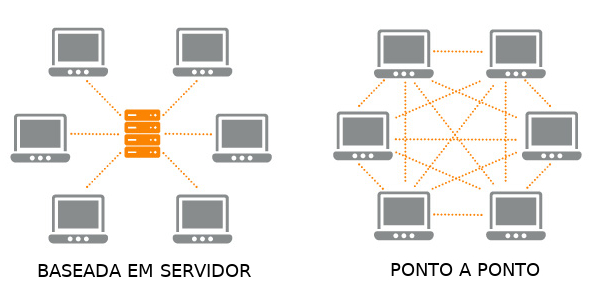
\includegraphics[width=\textwidth]{imagens/Server-based-vs-P2P-network.jpg}
	\caption{Rede com a arquitetura centralizada à esquerda e rede ponto a ponto à direita}
	Fonte: \cite{Wowza}
	\label{fig:redes}
\end{figure}

Na arquitetura centralizada, toda a rede fica dependente de um nó central, que fornecerá todos os recursos necessários para o funcionamento da rede. Esse nó detém todo o poder e controle, caso haja algum problema com ele, a rede ficará comprometida por completo. Já nas redes \textit{peer-to-peer}, isso não é um empecilho. Caso algum nó sofra com algum problema ou se desconecte voluntariamente da rede ou perca todas as informações, ninguém será afetado, todos continuarão realizando suas ações normalmente.

Apesar das vantagens, os sistemas ponto a ponto apresentam contrapartidas. Entre elas estão, principalmente, a integridade e confiança. Problemas estes que podem estar relacionados com falhas técnicas, nós mal intenciondos (usuários maliciosos), vulnerabilidade, integridade de informação, entre outros.
\section{Bitcoin}

O \textit{Bitcoin} geralmente é tratado como se fosse apenas uma moeda. Porém, o \textit{Bitcoin} é uma coleção de conceitos e tecnologias responsáveis por formar a base de todo um ecossistema um dinheiro digital. \cite{Antonopoulos2014} Dentro dessa variedade de conceitos que podem ser atribuídos a ele, podemos destacar três: (1) Um ativo digital (criptomoeda), (2) uma referência à tecnologia \textit{Blockchain} (livro-razão descentralizado) e (3) o protocolo que é executado sobre a tecnologia \textit{Blockchain} para descrever como os ativos são transferidos (\textit{softwares} que conduzem a transação) \cite{Swan2015}.

Todo esse sistema de pagamento de dinheiro digital foi lançado em 2009, sendo desenvolvido com um \textit{design} descentralizado e protegido por uma poderosa criptografia, tornando-o resiliente contra manipulações. \cite{Caetano2015} Os usuários possuem chaves que permitem com que eles provem a sua posse das moedas no decorrer das transações. Tais chaves são sempre armazenadas em uma carteira digital, a qual pode existir no computador do usuário, em sites de transações, em \textit{exchanges}, em \textit{hardwares}, ou em outras plataformas digitais. 

\section{Blockchain}

Assim, como o \textit{Bitcoin}, o \textit{Blockchain} também abrange um leque de significados, como: (1) uma terminologia para uma estrutura de dados, (2) o nome de um algoritmo, (3) um conjunto de tecnologias e (4) um termo abrangente para sistemas \textit{peer-to-peer} puramente distribuídos com uma área de aplicação comum.

Quando utilizado para nomear uma estrutura de dados, o termo refere-se a vários dados unidos em unidades chamadas de blocos. Tais blocos são conectados uns aos outros de forma encadeada, daí vem o nome \textit{Blockchain} (cadeia de blocos, em tradução livre). Quando atribuído a um algoritmo, o significado refere-se a um conjunto de instruções que lidam com o conteúdo de muitas estrutura de dados \textit{Blockchain} em um sistema \textit{p2p}. Ao se referir a um conjunto de tecnologias, o termo inclui a estrutura de dados, o algoritmo, tecnologias de criptografia e segurança os quais podem ser utilizados para prover integridade em sistemas puramente distribuídos ponto a ponto. E, diferente do significado anterior, a quarta atribuição ao termo é referente à um sistema distribuído como um todo, não unicamente a uma unidade de \textit{software} que faz parte desse tipo de sistema. \cite{Drescher2018}

O desenvolvimento desta tecnologia foi um avanço fundamental na ciência da computação, juntando cerca de quarenta anos de pesquisas em criptografia com vinte anos de pesquisas em moedas criptográficas. \cite{Swan2015} O Blockchain resolve um problema de longa data chamado “gasto duplo”. Este problema ocorre quando duas transações são aceitas com um montante que excede o valor antes disponível para gasto, ou seja, aquela quantia foi usada mais de uma vez.

Até o desenvolvimento do \textit{Blockchain}, o dinheiro digital não era escasso (assim como todos os outros recursos digitais), podendo ser copiados e replicados \textit{ad infinitum}, e não havia uma ­maneira de confirmar se aquele recurso já havia sido gasto sem que houvesse uma terceira parte envolvida para intermediar e realizar a sincronização entre todas as transações \cite{Swan2015}.

Para resolver o gasto duplo, o \textit{Blockchain} provê um mecanismo de confirmação e um livro-razão universal distribuído para que todos os nós (pontos) estejam informados e atualizados ao longo de cada transação. Cada informação nova adicionada na cadeia de blocos é armazenada em ordem cronológica, assim, fazendo com que o rastreamento seja feito de maneira simples. A cada 10 minutos um novo grupo de transações – ou seja, um bloco – é adicionado ao livro e todos os nós possuirão uma cópia do mesmo. Caso alguém tente usar o mesmo recurso mais de uma vez, será impossível, pois uma vez que a primeira operação dela foi iniciada, a mesma vai para um \textit{pool} de transações não confirmadas. Apenas a primeira das duas transações será confirmada e verificada pelos mineradores, enquanto a segunda será classificada como inválida e não terá confirmações suficientes para ser validada; e mesmo que as duas transações sejam feitas ao mesmo tempo, a que tiver mais confirmações dos mineradores (no mínimo seis, para que seis outros blocos sejam adicionados no topo do bloco que está sendo verificado) será a aceita.

A imagem abaixo mostra os passos para a realização de uma transação com \textit{Blockchain}. Primeiro, o usuário requisita uma transação. Em seguida, essa mesma requisição é transmitida para a rede, que será responsável por validar ou rejeitar o pedido de transação. Após isso, caso seja validada, ela é adicionada ao atual bloco de transações, o qual será encadeado com os outros blocos mais antigos, assim, confirmando a transação.

\begin{figure}[h]
	\centering
	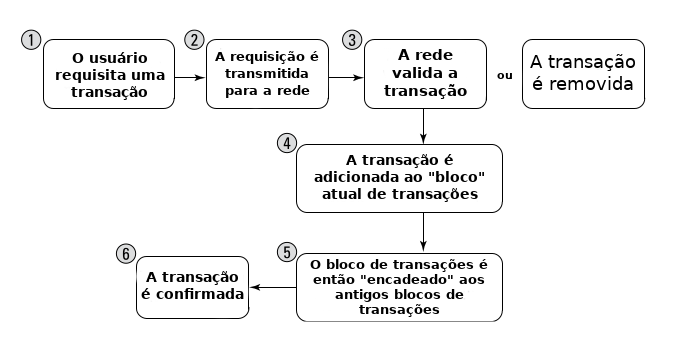
\includegraphics[width=\textwidth]{imagens/funcionamento-blockchain.png}
	\caption{Funcionamento do Blockchain}
	Fonte: \cite{Laurence2017}
	\label{fig:funcionamento-blockchain}
\end{figure}

A relação entre os sistemas \textit{p2p} e o \textit{Blockchain} é que o último serve para prover manter a integridade do primeiro sem que haja intermediação \cite{Drescher2018}.

\section{Exchanges}

As exchanges de criptoativos são plataformas digitais, com funcionamento
em tempo real que servem como intermediárias na compra, venda e troca dos mesmos, a fim de
facilitar o processo de aquisição. Elas costumam cobrar taxas nessas transações e organizar as 
informações de cada negociação em livros abertos. As exchanges são intermediários optativos, já
que, as criptomoedas podem funcionar de forma independente sem a necessidade de um intermediário envolvido no processo.

As seis \textit{exchanges} abordadas neste trabalho foram escolhidas com base no seu volume de transação e no nível de maturidade de sua \textit{API}. O volume é definido pela soma de todos os pares de mercado (\textit{market pairs}\footnote{\em Um \textit{market pair} é a cotação de duas moedas diferentes, com o valor de uma sendo cotado contra o valor de outra. O par é composto por uma moeda base e outra moeda de cotação.}) reportado pela corretora nas últimas vinte e quatro horas.

As informações a respeito do volume das corretoras são encontradas no \textit{Coin Market Cap}\footnote{\em https://coinmarketcap.com/rankings/exchanges/}, um \textit{site} que disponibiliza dados e gráficos em tempo real tanto das \textit{exchanges} quanto das criptomoedas existentes no mercado. No momento da escolha, as corretoras aqui analisadas estavam presentes entre as vinte primeiras posições no \textit{Coin Market Cap}.


\section{HTTP}

Projetado no início da década de 1990, o \textit{Hypertext Transfer Protocol} (Protocolo de Transferência de Hipertexto) é um protocolo de comunicação utilizado na transferência de documentos na \textit{Internet}. Ele garante a integridade dos dados transmitidos durante a comunicação. É por meio dele que as informações oriundas de servidores \textit{web} chegam de forma rápida, conveniente e confiável aos internautas, nos seus respectivos navegadores. O \textit{HTTP} segue o modelo de comunicação cliente-servidor, o qual o cliente inicia uma conexão com o servidor, realiza requisições e aguarda até receber alguma resposta.

\begin{figure}[h]
	\centering
	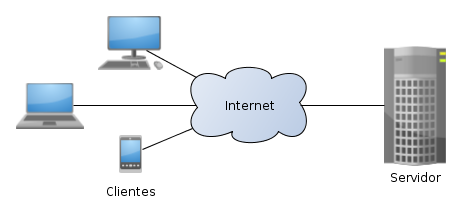
\includegraphics[width=\textwidth]{imagens/modelo-arquitetura-cliente-servidor.png}
	\caption{Modelo de arquitetura cliente-servidor}
	\cite{ClienteServidorWikipedia}
	\label{fig:modelo-arquitetura-cliente-servidor}
\end{figure}

\begin{figure}[h]
	\centering
	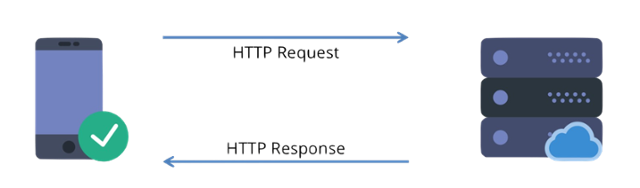
\includegraphics[width=\textwidth]{imagens/requisicao-http.png}
	\caption{Funcionamento de uma requisição HTTP}
	Fonte: \cite{HttpRequest}
	\label{fig:requisicao-http}
\end{figure}

Os servidores \textit{web} – também conhecidos como servidores \textit{HTTP} – são responsáveis por armazenar e prover todos os tipos de recursos \textit{web}: arquivos de texto, arquivos \textit{HTML}, arquivos de multimídia, etc.. O \textit{client} requisita ao \textit{server} o conteúdo desejado por meio de \textit{HTTP requests}  (requisições), e os servidores retornam os dados por meio de \textit{HTTP responses} (respostas) \cite{Gourley&Totty2002}, como mostrado na figura \ref{fig:requisicao-http}.

Além das características citadas, anteriormente, este protocolo é \textit{stateless}, ou seja, cada requisição é independente, mesmo que venham a ocorrer de forma simultânea e na mesma conexão cliente-servidor. Para o \textit{server}, cada \textit{request} é diferente, ele não guarda o estado das requisições anteriores, toda a informação é perdida.

\subsection{REST}

\textit{REST} é um acrônimo para \textit{Representational State Transfer} (Transferência de Estado Transacional), um estilo arquitetural para sistemas \textit{web} distribuídos a fim de facilitar a comunicação entre eles. Foi apresentado em 2000 por Roy Fielding, um dos autores da especificação do \textit{HTTP}, em sua tese de doutorado\footnote{\em https://www.ics.uci.edu/~fielding/pubs/dissertation/top.htm}. Nela, Roy sugeriu um conjunto de princípios, regras e \textit{constraints} que permitem o desenvolvimento de aplicações com interface bem definidas.
	
As aplicações desenvolvidas que seguem essa arquitetura são denominadas \textit{RESTful}, e seis princípios devem ser respeitados na implementação das mesmas:

\begin{itemize}
	\item \textbf{Cliente-servidor}: a portabilidade da interface do usuário e a escalabilidade do sistema  são melhoradas quando há uma separação do cliente, responsável pela interface, do servidor, que armazena as informações;
	\item \textbf{Stateless}: informações de sessão do usuário fica a cargo do cliente. Cada requisição para o servidor deve conter todas as informações necessárias para que ele entenda o \textit{request};
	\item \textbf{Armazenamento em cache}: requer que os dados em uma resposta sejam rotulados implícita ou explicitamente se podem ou não serem armazenados em \textit{cache}. Caso positivo, o cache do cliente poderá utilizar essas informações retornadas do servidor em outras requisições futuras;
	\item \textbf{Interface uniforme}: a fim de simplificar a arquitetura de todo o sistema, o \textit{REST} busca obter uma interface uniforme definindo quatro \textit{constraints}: identificação dos recursos, manipulação dos recursos através de representações, mensagens auto descritivas e hipermídia como motor do estado da aplicação;
	\item \textbf{Sistemas em camadas}: este modelo, também conhecido como \textit{layered systems}, permite que uma arquitetura seja composta de camadas hierárquicas, restringe o comportamento dos componentes de forma que cada um deles não possa acessar outras camadas além da qual eles estão interagindo no momento;
	\item \textbf{Código sob demanda}: este último princípio é optativo. Geralmente o usuário enviará as representações estáticas de recursos (\textit{JSON} ou \textit{XML}), porém, caso seja necessário, é possível retornar o código fonte executável para suportar parte da aplicação que está sendo desenvolvida.
\end{itemize}

\section{API}

\textit{Application Programming Interface} – Interface de Programação de Aplicações, em tradução livre – é um conjunto de definições, protocolos e ferramentas para o desenvolvimento e integração de \textit{softwares} de aplicações. Essa interface permite que o sistema possa se comunicar com produtos e serviços oferecidos por outras aplicações, dessa forma, simplificando e tornando mais flexível o processo de construção do sistema, consequentemente, gerando economia de tempo e de recursos.

Com as \textit{APIs}, a aplicação deixa disponível recursos, serviços e informações sem que haja uma perda na segurança e no controle, já que o acesso e as permissões serão especificadas pela equipe de desenvolvimento. Nos últimos anos, o \textit{REST} vem sendo o principal protocolo de padronização de \textit{APIs}.

\subsection{\textit{REST API: Design Rulebook}}

É o principal material utilizado neste trabalho como base para realizar as análises das \textit{APIs}. Segundo \cite{Masse:2016}, as regras servem para ajudar os desenvolvedores a construir \textit{RESTful APIs} consistentes que podem ser desfrutadas pelos usuários. Algumas delas tornaram-se padrões, de fato, outras era implícitas no protocolo \textit{HTTP}. Tais regras podem ser utilizadas por completo ou de forma separada, dependendo do contexto do serviço, e elas servem para responder algumas questões como:

\begin{itemize}
	\item Quando os caminhos da \textit{URI} devem ser nomeados com substantivos no plural?
	\item Quais métodos de requisição devem ser utilizados para atualizar o estado dos recursos?
	\item Como implementar operações diferentes do \textit{CRUD} nas \textit{URIs}?
	\item Qual é o código de \textit{status} \textit{HTTP} apropriado para um determinado cenário?
	\item Como gerenciar diferentes versões de uma representação do estado de um recurso?
	\item Como estruturar um \textit{hyperlink} em \textit{JSON}? 
\end{itemize}

\section{Trabalhos relacionados}

\subsection{\textit{API Management: An Architect’s Guide to Developing and Managing APIs for Your Organization}}

Este livro é um guia de como desenvolver, gerenciar e manter \textit{APIs} em sistemas corporativos. O autor aborda questões de segurança, ciclo de vida, documentação, padrões de projeto, controle de versão, monetização, \textit{analytics} e estratégias para testes de performance e testes de carga.

Na seção de seção de \textit{design} da interface da \textit{API}, princípios básicos do \textit{REST}, os verbos, os \textit{status codes}, a estrutura, convenções e boas práticas dos identificadores de recursos \textit{URIs}, versionamento, e outros detalhes importantes e necessários no projeto de construção de uma \textit{API}.

Segundo \cite{De2017}, as \textit{APIs} devem ser desenvolvidas para que tenham um longo ciclo de vida. Qualquer mudança acarreta em riscos de funcionamento para o cliente que a consome. Frequentes mudanças geralmente deixam usuários comuns e desenvolvedores frustrados. Utilizar padrões robustos na construção de \textit{APIs} ajuda a comunidade de desenvolvedores e pode salvar a companhia de ter despesas financeiras.

\subsection{\textit{REST API Development with Node.js: Manage and Understand the Full Capabilities of Successful REST Development}}

Assim como o trabalho anterior, neste livro o \cite{Doglio:2018} mostra todos os passos necessários para se desenvolver uma \textit{API} e lançá-la em um ambiente de produção. Nele, é feita uma introdução ao \textit{REST} e como desenvolver uma \textit{RESTful API} na linguagem \textit{Javascript} utilizando o \textit{framework Node.js}. A diferença encontra-se na abordagem das boas práticas de desenvolvimento de \textit{APIs}. O livro traz o conteúdo de forma mais superficial, não se aprofundando ou expondo os padrões minuciosamente. Por outro lado, o autor abordar o conteúdo didaticamente.

\subsection{\textit{API Design for C++}}

Este livro trata de forma mais profunda a construção de \textit{APIs} elegantes e robustas. Criar interfaces de alta qualidade é, portanto, uma habilidade essencial de engenharia e o foco central deste trabalho. \cite{Reddy2011}

Para auxiliar na performance, o autor utiliza a linguagem de programação \textit{C++}, que permite que a aplicação seja processada até mesmo em unidades de processamento gráfico (GPU). Alguns componentes para aumentar o desempenho das \textit{APIs} são considerados, entre eles: velocidade do tempo de compilação, velocidade do tempo de execução, sobrecarga da memória em tempo de execução, tamanho da aplicação e o tempo de inicialização.

Além do desempenho da aplicação, o livro aborda os diferentes tipos de \textit{patterns} de implementação e possui uma seção que trata da qualidade de uma \textit{API}, descrevendo as caracteríticas que uma boa aplicação deve ter, entre elas: modelagem do domínio do problema, esconder os detalhes de implementação, ser fácil de utilização, ser testada, documentada e estável.

  \chapter{Análise das \textit{APIs} das \textit{exchanges}}
\label{chap:desenvolvimento}

Neste capítulo são realizadas todas as análises das \textit{APIs} das corretoras de criptomoedas, baseando-se em trinta e três regras retiradas do livro \textit{REST API: Design Rulebooks} e nas limitações de uso definidas pelas próprias \textit{exchanges} na documentação de suas respectivas \textit{API}.

\section{Ferramentas utilizadas}

Nesta pesquisa foram usadas algumas ferramentas para auxiliar no processo de consulta e análise das requisições e respostas das \textit{APIs}.

\subsection{Postman}
O \textit{Postman} é uma aplicação desenvolvida com a finalidade de realizar diversos tipo de testes em \textit{APIs RESTful}. Através da sua interface, é possível enviar requisições \textit{HTTP}, analisar os resultados, consultar informações mais detalhadas e ter uma visão mais aprofundada do funcionamento dos serviços que estão sob consulta. Esta plataforma também possibilita que os desenvolvedores documentem as suas \textit{APIs} e possam planejar e escrever casos de testes.

Na imagem abaixo temos um exemplo do uso da ferramenta neste trabalho. Nele, inserimos a \textit{URI} e selecionamos o verbo \textit{HTTP} e realizamos a requisição. O \textit{software} exibirá na sua interface a resposta da requisição formatada, o cabeçalho do \textit{response}, informações do tempo de duração e do tamanho da resposta, \textit{status ode}, entre outros.
\begin{figure}[h]
	\centering
	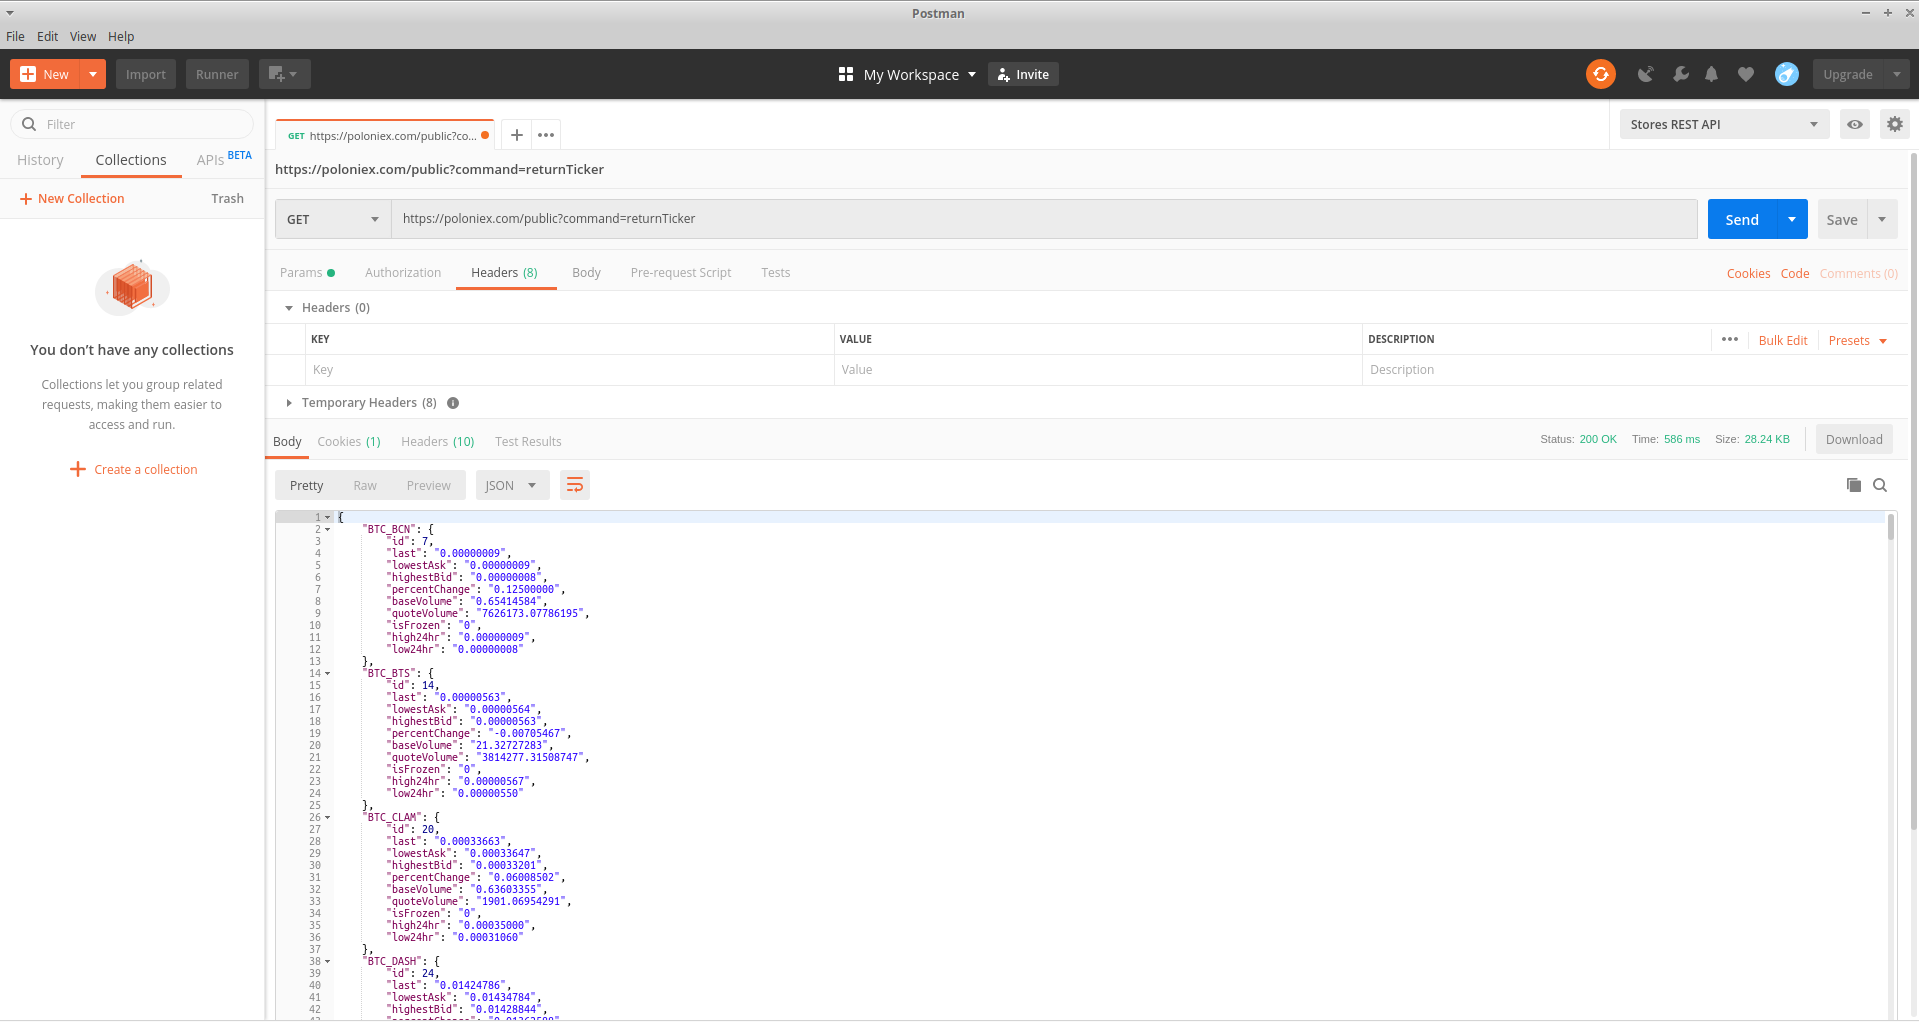
\includegraphics[width=\textwidth]{imagens/postman.png}
	\caption{Interface do Postman}
	\label{fig:postman}
\end{figure}

\subsection{Google Chrome}
O navegador Google Chrome disponibiliza em seu próprio \textit{software} as "Ferramentas de desenvolvedor", as quais permitem ao usuário analisarem uma gama de recursos e conteúdos de uma página na \textit{Internet}. Com elas, é possível ver e editar o código-fonte da página, acessar os arquivos e recursos da aplicação, visualizar as informações e dados enviadas na requisição e recebidos na resposta além de mensagens de erros, monitorar o tráfego \textit{HTTP}, depurar códigos desenvolvidos na linguagem \textit{JavaScript}, acessar informações do uso de memória e fontes de latência, entre outros.

\begin{figure}[h]
	\centering
	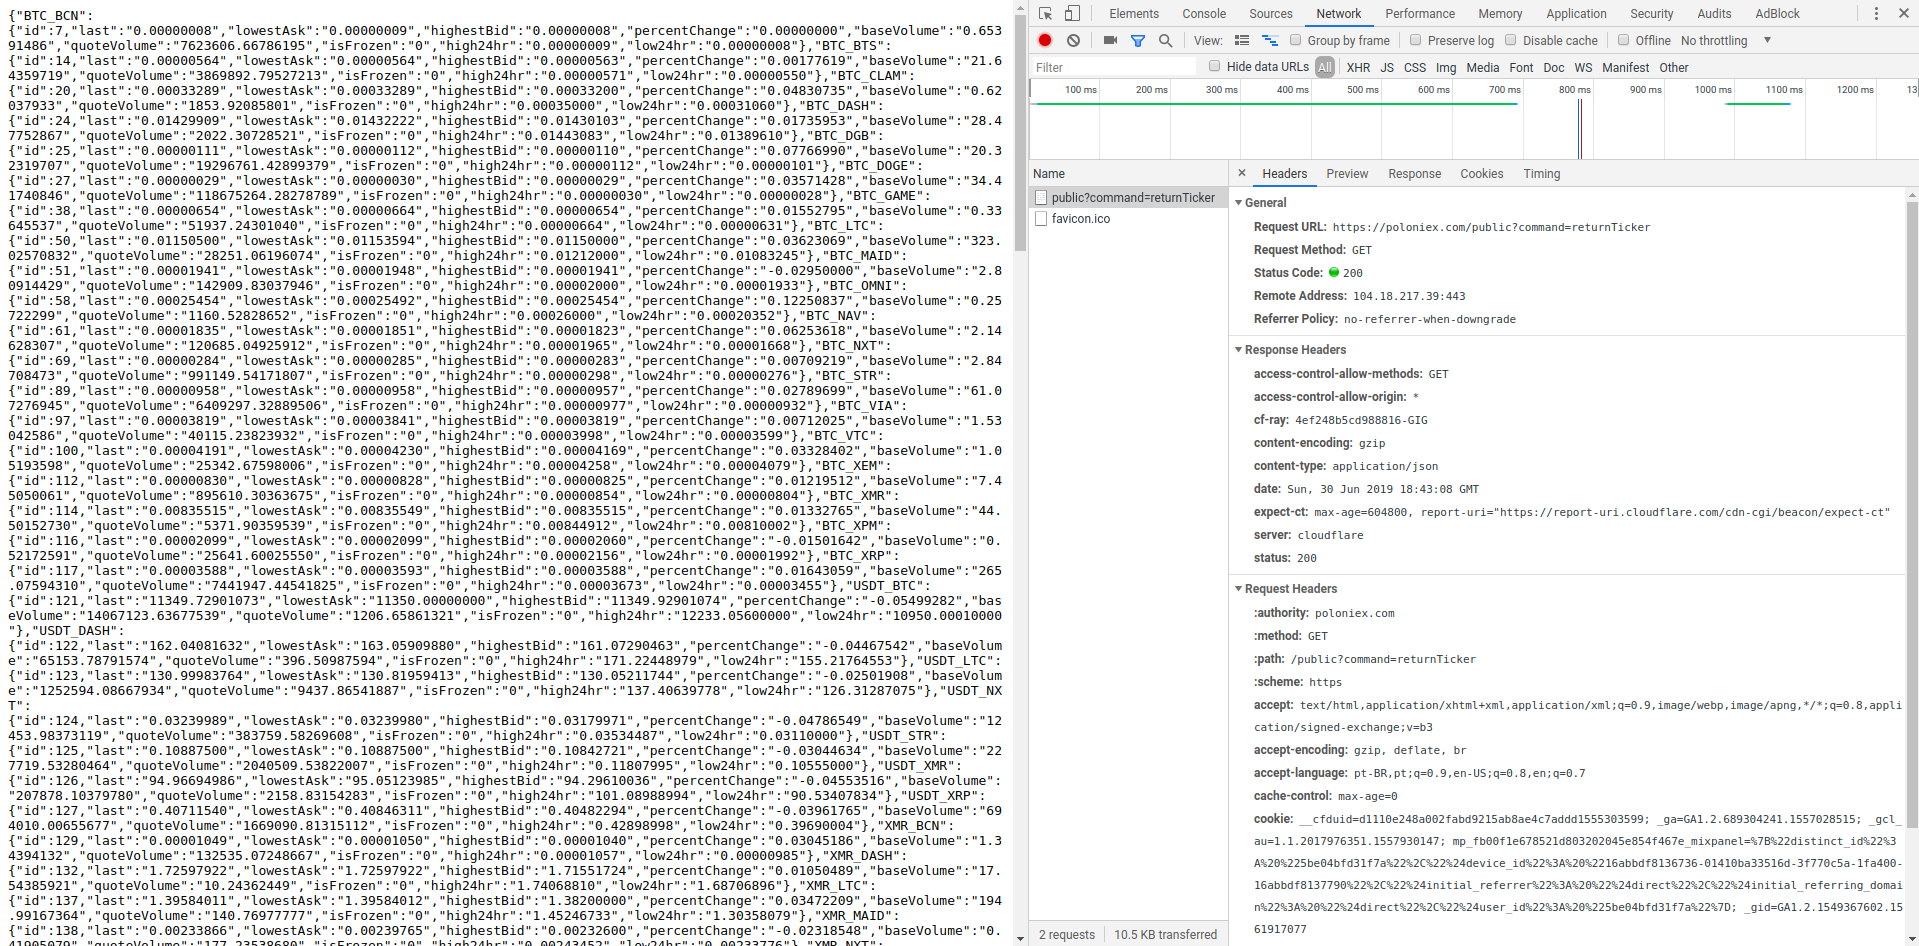
\includegraphics[width=\textwidth]{imagens/google1.png}
	\caption{Interface das Ferramentas de desenvolvedor}
	\label{fig:google}
\end{figure}

No exemplo acima é mostrado como uma requisição é feita pelo navegador e como as suas informações são dispostas na interface. No lado esquerdo a resposta é exibida ao usuário, já o lado oposto é composto pela ferramenta de desenvolvedor, com detalhes da requisição e da reposta, informações gerais - \textit{URL}, método \textit{HTTP}, \textit{status code}, etc. -, cabeçalhos do \textit{request} e do \textit{response}, além da possibilidade de ver possíveis mensagens de erro na aba \textit{Console}, informações a respeito da rede na aba \textit{Network} e dados de memória e performance.

\subsection{CURL}
O \textit{Client URL} é uma ferramenta de linha de comando, podendo também ser utilizada em \textit{scripts}, presente nos Sistemas Operacionais baseados em \textit{Unix}, e são destinados a verificar a conectividade da \textit{URL}, podendo ser utilizado também para realizar transferência de dados. Ele suporta vários protocolos utilizados na \textit{Internet}, dentre eles o \textit{HTTP}.

Em determinadas \textit{exchanges}, para acessar as rotas privadas é necessário que haja um código criptografado que é gerado através da chave privada da \textit{API}, do comando desejado e da data e hora atual em milissegundos (\textit{nonce}), utilizando o algoritmo de criptografia \textit{hash SHA-512}.   
\begin{figure}[h]
	\centering
	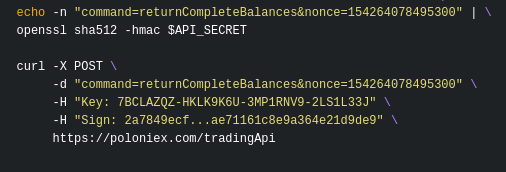
\includegraphics[width=\textwidth]{imagens/curl1.png}
	\caption{Uso do cURL}
	\label{fig:google}
\end{figure}

\section{Regras selecionadas}

\subsection{Modelagem de identificadores com \textit{URIs}}

O Identificador de Recursos Universal, ou \textit{URI} - Unified Resource Language - é um elemento presente nas \textit{APIs REST}. O mesmo é utilizado para endereçar recursos. Cada recurso deve possuir um nome significativo para que o mesmo seja identificado.
Modelá-los é uma das mais importantes tarefas para o sucesso de uma \textit{API}, sendo responsável por deixá-la mais intuitiva e de fácil manuseio para os seus usuários \cite{De2017}.

\subsubsection{Formato da \textit{URI}}

O formato de uma \textit{URI} deve seguir a seguinte estrutura abaixo:

\centerline{\textbf{esquema} "://" \textbf{autoridade} "/" \textbf{caminho} [ "?" \textbf{consulta} ] [ "\#" \textbf{fragmento} ]}

\begin{itemize}
    \item \textbf{Esquema:} É o espaço utilizado para identificar o protocolo que está sendo utilizado. Por exemplo: \textit{HTTP, HTTPS, FTP}, etc;
    \item \textbf{Autoridade:} Representa a resolução do \textit{Domain Name System} do servidor em que a aplicação está sendo executada. Pode ser composta pelo \textit{hostname} ou pelo endereço de \textit{IP}, opcionalmente com o número da porta ou com credenciais de acesso;
    \item \textbf{Caminho:} Determina uma sequência de segmentos dipostos de forma hierárquica e separados por uma barra (/);
    \item \textbf{Consulta:} São informações adicionais, não hierárquicas, de identificação. Sempre são precedidas de uma interrogação;
    \item \textbf{Fragmento:} São separados por cerquilhas (\#) e direcionam para recursos secundários dentro dos recurso primário, o qual é identificado pela autoridade.
\end{itemize}

\textbf{Regra 1 - O separador (/) deve ser usada para indicar relacionamento hierárquico.}

\begin{itemize}
    \item \textbf{Binance:} apesar de seguir a regra, algumas rotas poderiam ter uma hierarquia organizada de forma mais eficiente. Por exemplo: as rotas \textit{/api/v3/openOrders} e \textit{/api/v3/allOrders} deveriam ser atreladas a um \textit{endpoint /orders/}, que retornaria todas as ordens, e com a possibilidade eu filtrar a ordem pelo \textit{status} (aberta, finalizada, cancelada, etc.) em uma \textit{query}.
    \item \textbf{Bittrex:} utiliza a regra de forma coerente.
    \item \textbf{Poloniex:} não trabalha com hierarquia, todos os comandos são executados por meio de uma \textit{query} ou por meio do corpo da requisição utilizando \textit{JSON}.
    \item \textbf{Livecoin:} a hierarquia deveria ser melhor estruturada. Por exemplo: para as rotas \textit{/exchange/buylimit} e \textit{/exchange/selllimit}, o correto seria ter um caminho \textit{/exchange/limit} e eu escolher o tipo (\textit{buy} ou \textit{sell}) por consulta, por meio do corpo da mensagem via \textit{JSON} ou, até mesmo, criando mais duas rotas \textit{/exchange/limit/buy} e \textit{/exchange/limit/sell}.
    \item \textbf{Gate.io:} assim como na Binance e na Livecoin, o problema com a organização da hierarquia se repete. Rotas como \textit{/private/cancelOrders} e \textit{/private/cancellAllOrders} poderiam ser provenientes da hierarquia \textit{/private/orders}.
    \item \textbf{Huobi:} utiliza a regra de forma coerente.
\end{itemize}

\textbf{Regra 2 - O separador (/) não deve ser incluída no final da \textit{URI}:} o acréscimo deste elemento não adiciona nenhum conteúdo semântico e pode causar confusão.

Todas as corretoras cumprem esta regra.

\textbf{Regra 3 - Hífens (-) devem ser utilizados para melhorar a legibilidade da \textit{URI}.}

\begin{itemize}
    \item \textbf{Binance:} utiliza o padrão \textit{camelCase}, onde a primeira palavra inicia com letra minúscula e as demais com letra maiúscula.
    \item \textbf{Bittrex:} não separa as palavras.
    \item \textbf{Poloniex:} utiliza o padrão \textit{camelCase}.
    \item \textbf{Livecoin:} não possui um padrão, em determinados \textit{endpoints} faz a separação com sublinha (\_), enquanto outros são separados com o padrão \textit{camelCase}.
    \item \textbf{Gate.io:} não tem um padrão definido, alterna entre sublinhas e \textit{camelCase}.
    \item \textbf{Huobi:} padronizada com o \textit{camelCase}.
\end{itemize}

\textbf{Regra 4 - Sublinhas (\_) não devem ser usadas nas \textit{URIs}:} geralmente, aplicações de visualização de texto utilizam a sublinha para indicar que aquele elemento é clicável. Além disso, dependendo da fonte utilizada na aplicação, a sublinha pode ficar escondida ou de difícil visualização.

Como mostrado na regra de número 3, as corretoras Livecoin e Gate.io fazem uso das sublinhas, dessa forma ambas não cumprem a regra.

\textbf{Regra 5 - Letras minúsculas devem ser preferidas em caminhos da \textit{URI}:} A \textit{RFC} 3986\footnote{\em https://www.ietf.org/rfc/rfc3986.txt} define que as \textit{URIs} são \textit{case-sensitive}, ou seja, diferenciam letras minúsculas e maiúsculas nos componentes do Identificador de Recurso Universal (com exceção do esquema e da autoridade).

Apenas a Bittrex utiliza letras minúsculas em todas as suas rotas.

\textbf{Regra 6 - Extensões de arquivos não devem ser inclusas nas \textit{URIs}.} Todas as \textit{exchanges} cumprem esta regra nas suas \textit{APIs}.

\subsubsection{Modelagem de autoridade da \textit{URI}}

\textbf{Regra 7 - Nomes de subdomínios consistentes devem ser utilizados:} os nomes do domínio de alto nível e do primeiro subdomínio (ex.: ifrn.edu.br) de uma \textit{API} deve identificar o proprietário do serviço ofertado. O nome completo deve incluir um subdomínio chamado \textbf{api}, como na estrutura a seguir.

\centerline{https://api.ifrn.edu.br}

\begin{itemize}
    \item \textbf{Binance:} cumpre a regra.
    \item \textbf{Bittrex:} cumpre a regra.
    \item \textbf{Poloniex:} não segue o padrão \textit{api.subdominio}, além de possuir duas ramificações na \textit{URI}, uma para a api pública (\textit{poloniex.com/public}) e outra para a privada (\textit{poloniex.com/tradingApi}).
    \item \textbf{Livecoin:} cumpre a regra.
    \item \textbf{Gate.io:} tem quatro subdomínios, dados para os dados públicos (\textit{data.gateio.co/api2/1} e \textit{data.gateio.io/api2/1}) e mais dois para informações privadas (\textit{api.gateio.co/api2/1/private} e \textit{api.gateio.io/api2/1/private}).
    \item \textbf{Huobi:} cumpre a regra.
\end{itemize}

\subsubsection{Resumo}

\begin{table}[h]
    \centering
    \begin{tabular}{|c|c|c|c|c|c|c|}
        \hline
        \textbf{Regras} & \textbf{Binance} & \textbf{Bittrex} & \textbf{Poloniex} & \textbf{Livecoin} & \textbf{Gate.io} & \textbf{Huobi} \\ \hline
        Regra 1         & Parcialmente             & Sim                & Não                 & Parcialmente               & Parcialmente              & Sim             \\ \hline
        Regra 2         & Sim                & Sim                & Sim                 & Sim                 & Sim                & Sim              \\ \hline
        Regra 3         & Não                & Não                & Não                 & Não                 & Não                & Não              \\ \hline
        Regra 4         & Sim                & Sim                & Sim                 & Não                 & Não                & Sim              \\ \hline
        Regra 5         & Parcialmente              & Não                & Parcialmente               & Parcialmente               & Parcialmente              & Parcialmente            \\ \hline
        Regra 6         & Sim                & Sim                & Sim                 & Sim                 & Sim                & Sim              \\ \hline
        Regra 7         & Sim                & Sim                & Não                 & Sim                 & Não                & Sim              \\ \hline
    \end{tabular}
    \caption{Cumprimento das regras de modelagem de identificadores com \textit{URI} por \textit{exchange}}
    \label{tab:table-1}
\end{table}

A Huobi foi a \textit{exchange que mais seguiu os padrões de modelagem de \textit{URI}}, cumprindo cinco regras e descumprindo apenas uma. Em seguida temos a Bittrex e a Binance cumprindo cinco e quatro regras, respectivamente. As demais corretoras não tiveram um bom desempenho nessa análise, cumprindo menos de quatro regras.

É notável que nenhuma das \textit{exchanges} seguiu a terceira regra. Todas optaram por utilizar o padrão \textit{camelCase} ao invés de utilizar a separação por hífens. Apesar disso, essa violação não causará impacto na utilização das \textit{APIs}.

\subsection{Modelagem de recursos}

A modelagem de recursos é um processo semelhante à modelagem de dados em bancos relacional. Ela é ajuda a fixar alguns conceitos-chave no desenvolvimento da \textit{API}.
É de demasiada importância escolher os recursos certos e modelá-los minuciosamente, para que os consumidores da aplicação possam receber as funcionalidades, comportamentos e manutenções desejadas \cite{Subramaniam2014}.

De forma similar aos padrões de projeto (\textit{design patterns}), o projeto de recursos de uma \textit{API} é composto por quatro \textbf{arquétipos de recursos} (documento, coleção, armazenamento e controlador), os quais ajudam a comunicação se tornar mais consistente entre as estruturas e comportamentos comuns.

\begin{itemize}
    \item \textbf{Documento (\textit{document}):} representa um único recurso dentro de uma coleção. É um conceito singular semelhante a uma instância de um objeto ou registro em um banco de dados;
    \item \textbf{Coleção (\textit{collection}):} equivale a um diretório de recursos gerenciado pelo servidor. Recursos adicionais podem ser inseridos pelos usuários caso seja permitido pela coleção;
    \item \textbf{Reserva (\textit{store}):} diferente das coleções, uma reservas é um repositório de recursos gerenciado pelo cliente;
    \item \textbf{Controlador (\textit{controller}):} controladores são equivalentes à funções executáveis, possuindo parâmetros, valores de retorno, dados de entrada e de saída.
\end{itemize}

\subsubsection{Modelagem do caminho da \textit{URI}}

\textbf{Regra 8 - Substantivo no plural devem ser utilizados para nomes de coleções.}

Todas as corretoras seguem esta regra, porém, a Poloniex utilizam um padrão de nomeação das rotas que retornam coleções semelhante a uma função na programação, por exemplo: \textit{returnBalances, returnOpenOrders}.

\textbf{Regra 9 - Um verbo ou uma frase verbal deve ser utilizada para nome de controladores.}

A Binance é a única que, em algumas rotas, como a \textit{/api/v3/order}, não há um verbo ou uma frase verbal para executar controladores; no exemplo citado, para criar ou remover uma ordem.

\textbf{Regra 10 - Nomes de funções \textit{CRUD} não devem ser utilizados na \textit{URI}:} identificadores devem ser utilizados para indicar apenas recursos, nunca para indicar que funções de criar, ler, atualizar e deletar conteúdos (\textit{CRUD - create, read, update, delete}) estão sendo utilizadas.

Todas as corretoras seguiram esta regra no desenvolvimento de suas \textit{APIs}.

\subsubsection{Resumo}

Todas as corretoras cumpriram as regras de modelagem de recursos, com exceção da Binance que cumpre parcialmente a nona regra. Tal cumprimento ocorre devido ao fato das \textit{APIs} das \textit{exchanges} compartilharem funções, recursos e informações semelhantes.

\begin{table}[h]
    \centering
    \begin{tabular}{|c|c|c|c|c|c|c|}
        \hline
        \textbf{Regras} & \textbf{Binance} & \textbf{Bittrex} & \textbf{Poloniex} & \textbf{Livecoin} & \textbf{Gate.io} & \textbf{Huobi} \\ \hline
        Regra 8         & Sim                & Sim                & Sim                 & Sim                 & Sim                & Sim              \\ \hline
        Regra 9         & Parcialmente       & Sim                & Sim                 & Sim                 & Sim                & Sim              \\ \hline
        Regra 10        & Sim                & Sim                & Sim                 & Sim                 & Sim                & Sim              \\ \hline
        
    \end{tabular}
    \caption{Cumprimento das regras de modelagem de recursos por \textit{exchange}}
    \label{tab:table-2}
\end{table}

 
\subsection{Modelagem de consulta da \textit{URI}}

O componente de consulta (\textit{query}) é opcional em uma \textit{URI}. O mesmo contém um conjunto de parâmetros para serem interpretados como uma variação ou derivação do recurso determinado no caminho hierárquico do identificador. Ele fornece uma interação adicional entre o usuário e a \textit{API}, como a procura por termos específicos e filtros.

\textbf{Regra 11 - O componente de consulta de uma \textit{URI} pode ser utilizado para filtrar coleções ou reservas:} no exemplo abaixo temos uma forma de utilizar as \textit{queries} para filtrar a busca por uma coleção através de um valor específico.

\centerline{https://api.ifrn.edu.br/alunos?curso=informatica}

A regra foi cumprida por todas as \textit{exchanges}.

\textbf{Regra 12 - O componente de consulta de uma \textit{URI} dever ser usado para paginar coleções ou \textit{stores}:} o cliente deve ser capaz de utilizar as \textit{queries} para retornar coleções paginadas e resultados de reservas com os parâmetros \textit{pageSize} e \textit{pageStartIndex}, indicando a quantidade máxima de conteúdo desejado por consulta e o índice do primeiro elemento.

\centerline{https://api.ifrn.edu.br/alunos?pageSize=10\&pageStartIndex=20}

No exemplo mostrado acima, a \textit{API} retornará dez elementos, com o primeiro sendo equivalente ao vigésimo em uma consulta sem filtros de paginação, ou seja, o índice inicial será vinte.

Das seis corretoras, apenas a Binance faz uso do \textit{limit} para delimitar a quantidade de elementos retornados, mas não há \textit{queries} para paginar os resultados.

\subsubsection{Resumo}

A décima primeira regra foi cumprida por todas as \textit{exchanges}, porém, a última dessa seção, não o foi.

Há alguns motivos para os desenvolvedores dessas \textit{APIs} não se preocuparem com paginações, entre eles: a limitação geralmente ocorre utilizando-se outras informações - nome da moeda, a data e hora, etc. -, e, também, porque em algumas rotas os dados retornados em tempo real podem variar a cada milésimo de segundo e, dependendo da finalidade de quem consome a \textit{API}, o retorno de apenas uma amostra de todo o conjunto de dados pode interferir no resultado desejado, dessa forma, é melhor e mais fácil disponibilizar toda a massa de dados. 

\begin{table}[h]
    \centering
    \begin{tabular}{|c|c|c|c|c|c|c|}
        \hline
        \textbf{Regras} & \textbf{Binance} & \textbf{Bittrex} & \textbf{Poloniex} & \textbf{Livecoin} & \textbf{Gate.io} & \textbf{Huobi} \\ \hline
        Regra 11        & Sim              & Sim              & Sim               & Sim               & Sim              & Sim            \\ \hline
        Regra 12        & Não              & Não              & Não               & Não               & Não              & Não            \\ \hline
    \end{tabular}
    \caption{Cumprimento das regras de modelagem de consulta de \textit{URI} por \textit{exchange}}
    \label{tab:table-3}
\end{table}


\subsection{Modelagem de interação com \textit{HTTP}}

\textit{RESTful APIs} suportam todos os elementos e aspectos do protocolo \textit{HTTP} na sua versão 1.1, como os métodos de requisição - popularmente conhecidos como verbos \textit{HTTP} -, códigos de resposta e cabeçalhos.


\subsubsection{Métodos de requisição}

O \textit{HTTP} é composto por oito verbos:

\begin{itemize}
    \item \textit{\textbf{GET:}} utilizado para recuperar dados e informações;
    \item \textit{\textbf{POST:}} tem como função enviar dados para o servidor;
    \item \textit{\textbf{PUT:}} substitui todas as informações do recurso destinado com o conteúdo submetido;
    \item \textit{\textbf{PATCH:}} similar ao \textit{PUT}, a diferença é que o \textit{PATCH} faz uma atualização parcial de um recurso, ou seja, apenas alguns atributos do recurso em questão podem ser especificados para atualização;
    \item \textit{\textbf{HEAD:}} possui a mesma funcionalidade do método \textit{GET}, porém, o servidor deve retornar na resposta apenas o cabeçalho e o \textit{status} e não o corpo da mensagem;
    \item \textit{\textbf{DELETE:}} remove a representação do recurso alvo;
    \item \textit{\textbf{OPTIONS:}} descreve as opções de comunicação com o recurso alvo;
    \item \textit{\textbf{CONNECT:}} inicia a comunicação bidirecional com o recurso alvo, estabelecendo um túnel com o servidor;
    \item \textit{\textbf{TRACE:}} realizar um teste, enviando uma mensagem pelo caminho até o recurso alvo e o servidor respondendo a mensagem recebida.
\end{itemize}

\textbf{Regra 13 - \textit{GET} deve ser utilizada para recuperar a representação de um recurso.}

Todas as \textit{exchanges} seguem a regra, a única observação é a respeito da Bittrex, que utiliza apenas o \textit{GET} para todas as rotas.

\textbf{Regra 14 - \textit{GET} e \textit{POST} não devem ser usados no lugar de outros métodos de requisição.}

\begin{itemize}
    \item \textbf{Binance:} utiliza corretamente ambos os verbos.
    \item \textbf{Bittrex:} utiliza o \textit{GET} para todas as requisições.
    \item \textbf{Poloniex:} usa o \textit{GET} corretamente, mas o \textit{POST} é utilizado no lugar do \textit{DELETE}.
    \item \textbf{Livecoin:} usa o \textit{GET} corretamente, porém, o \textit{DELETE} é substituído pelo \textit{POST}.
    \item \textbf{Gate.io:} usa o \textit{GET} corretamente, mas o \textit{POST} é utilizado no lugar do \textit{DELETE}.
    \item \textbf{Huobi:} usa o \textit{GET} corretamente, porém, o \textit{DELETE} é substituído pelo \textit{POST}.
\end{itemize}

\textbf{Regra 15 - \textit{POST} deve ser usado para criar novos recursos em uma \textit{collection}.}

A única exceção à esta regra é a Bittrex, pelo motivo citado nas duas últimas regras.

\textbf{Regra 16 - \textit{POST} deve ser utilizado para executar controladores.}

A Bittrex é a única que não cumpriu.

\textbf{Regra 17 - \textit{DELETE} deve ser utilizado para remover um recurso.}

Apenas a Binance cumpriu a regra. Todas as outras atribuíram esta funcionalidade ao \textit{GET} ou ao \textit{POST}.

\subsubsection{\textit{Status codes} de resposta}

O protocolo \textit{HTTP} define uma gama de códigos de estado para que sejam usados a fim de transmitir para o cliente os resultados de uma requisição. Os \textit{status codes} são subdivididos em cinco categorias:

\begin{itemize}
    \item \textbf{Informacionais:} retorna informações de transferência a nível de protocolo. Sempre iniciam com o número 1;
    \item \textbf{Sucesso:} indica que a requisição foi aceita com sucesso. Iniciam com o número 2;
    \item \textbf{Redirecionamento:} informa ao cliente que ele deve executar mais ações para que sua requisição seja completada. Os códigos desta categoria começam com o número 3;
    \item \textbf{Erro no cliente:} indica que o erro na resquisição aconteceu do lado do cliente. Sempre iniciam com o número 4;
    \item \textbf{Erro no servidor:} indica que o erro na resquisição aconteceu do lado do servidor. Sempre iniciam com o número 5;
\end{itemize}

\textbf{Regra 18 - 200 (\textit{"Ok"}) deve ser usado para indicar sucesso não específico.}

Regra cumprida pelas \textit{APIs} de todas as \textit{exchanges}.

\textbf{Regra 19 - 200 (\textit{"OK}) não deve ser utilizado para comunicar erros no corpo da resposta.}

\begin{itemize}
    \item \textbf{Binance:} respeita a regra, retorando o código de erro equivalente ao problema e uma mensagem com um código de erro próprio e uma descrição.
    \item \textbf{Bittrex:} em alguns casos retorna o código 200.
    \item \textbf{Poloniex:} retorna 200, violando a regra.
    \item \textbf{Livecoin:} retorna 200, apesar de informar no corpo da \textit{response} um código de erro próprio.
    \item \textbf{Gate.io:} retorna 200, apesar de informar no corpo da \textit{response} um código de erro próprio.
    \item \textbf{Huobi:} retorna 200, apesar de informar no corpo da \textit{response} um código de erro próprio no formato texto.
\end{itemize}

\textbf{Regra 20 - 204 (\textit{"No Content"}) deve ser utilizado quando o corpo da resposta está intencionalmente vazio.}

Todas retornam o \textit{status code} 200. Apesar da Bittrex ser a única que não retorna uma mensagem vazia, ao contrário das outras, apenas um campo chamado \textit{"data"} é retornado vazio, o corpo da mensagem vem com outras informações além deste campo. Mesmo assim, a Bittrex, semelhante às demais, não cumpriu a regra.

\textbf{Regra 21 - 302 (\textit{"Found"}) não deve ser utilizado.}

Nenhuma \textit{exchange} utilizou este código nos cabeçalhos da resposta.

\textbf{Regra 22 - 400 (\textit{"Bad Request"}) pode ser usado para indicar falha não específica.}

A Binance, a Livecoin e a Huobi utilizam o \textit{Bad Request}. As demais retornam uma mensagem de erro no corpo equivalente, mas com \textit{status code} igual a 200.

\textbf{Regra 23 - 401 (\textit{"Unauthorized"}) deve ser usado quando há um problema com as credenciais do cliente.}

Somente a Binance respeita a regra do código 401. A Livecoin retorna o código 400, que seria equivalente ao \textit{"Not Found"} e as demais o código 200.

\textbf{Regra 24 - 404 (\textit{"Not Found"}) deve ser usado quando a \textit{URI} do cliente não pôde ser mapeada.}

De todas as \textit{exchanges}, a Binance, a Livecoin e a Huobi utilizam corretamente o código 404.

\textbf{Regra 25 - 405 (\textit{"Method Not Allowed"}) dever ser utilizado quando o método \textit{HTTP} selecionado não é suportado ou permitido.}

\begin{itemize}
    \item \textbf{Binance:} utiliza o código 404 (\textit{"Not Found"}).
    \item \textbf{Bittrex:} permite que vários métodos sejam executados em um \textit{endpoint}.
    \item \textbf{Poloniex:} permite que vários métodos sejam executados em um \textit{endpoint}.
    \item \textbf{Livecoin:} usa corretamente o código 405.
    \item \textbf{Gate.io:} usa corretamente o código 405.
    \item \textbf{Huobi:} permite que vários métodos sejam executados em um \textit{endpoint}.
\end{itemize}

\textbf{Regra 26 - 500 (\textit{"Internal Server Error"}) deve ser utilizado para indicar algum mal funcionamento da \textit{API}.}

\begin{itemize}
    \item \textbf{Binance:} retorna o \textit{status code} coerentemente, além de possuir outros códigos próprios para indicar diferentes tipos de erros internos no corpo da mensagem.
    \item \textbf{Bittrex:} faz uso da regra de forma correta.
    \item \textbf{Poloniex:} utiliza o código 200 e uma mensagem de erro própria.
    \item \textbf{Livecoin:} retorna uma código próprio e uma descrição no corpo da mensagem.
    \item \textbf{Gate.io:} retorna uma código próprio e uma descrição no corpo da mensagem.
    \item \textbf{Huobi:} utiliza o código 200.
\end{itemize}

\subsubsection{Resumo}

A \textit{exchange} que mais respeitou as regras de interação com o protocolo \textit{HTTP} foi a Binance, descumprindo apenas duas regras. A Bittrex obteve o pior desempenho descumprindo nove regras. Todas as demais descumpriram pelo menos cinco regras.

É perceptível que as corretoras ainda estão imaturas a respeito do tratamento de códigos de resposta \textit{HTTP}. Os usuários que consumirão essas \textit{APIs} somente em alguns casos poderão depender do \textit{status code} para saber sobre o estado da requisição, dependendo da corretora que forem trabalhar, terão que consultar o conteúdo retornado no corpo da mensagem, podendo tornar o desenvolvimento menos simples. 

\begin{table}[h]
    \centering
    \begin{tabular}{|c|c|c|c|c|c|c|}
        \hline
        \textbf{Regras} & \textbf{Binance} & \textbf{Bittrex} & \textbf{Poloniex} & \textbf{Livecoin} & \textbf{Gate.io} & \textbf{Huobi} \\ \hline
        Regra 13        & Sim                & Parcialmente       & Sim               & Sim                 & Sim                & Sim              \\ \hline
        Regra 14        & Sim                & Não                & Parcialmente      & Parcialmente        & Parcialmente       & Parcialmente     \\ \hline
        Regra 15        & Sim                & Não                & Sim               & Sim                 & Sim                & Sim              \\ \hline
        Regra 16        & Sim                & Não                & Sim               & Sim                 & Sim                & Sim              \\ \hline
        Regra 17        & Sim                & Não                & Não               & Não                 & Não                & Não              \\ \hline
        Regra 18        & Sim                & Sim                & Sim               & Sim                 & Sim                & Sim              \\ \hline
        Regra 19        & Sim                & Sim                & Não               & Não                 & Não                & Não              \\ \hline
        Regra 20        & Não                & Não                & Não               & Não                 & Não                & Não              \\ \hline
        Regra 21        & Sim                & Sim                & Sim               & Sim                 & Sim                & Sim              \\ \hline
        Regra 22        & Sim                & Não                & Não               & Sim                 & Não                & Sim              \\ \hline
        Regra 23        & Sim                & Não                & Não               & Não                 & Não                & Não              \\ \hline
        Regra 24        & Sim                & Não                & Não               & Sim                 & Não                & Sim              \\ \hline
        Regra 25        & Não                & Não                & Não               & Sim                 & Sim                & Não              \\ \hline
        Regra 26        & Sim                & Sim                & Não               & Não                 & Não                & Não              \\ \hline
    \end{tabular}
    \caption{Cumprimento das regras de modelagem de interação com \textit{HTTP} por \textit{exchange}}
    \label{tab:table-4}
\end{table}

\subsection{Modelagem de metadados}

\subsubsection{Cabeçalhos \textit{HTTP}}

Um conjunto de cabeçalhos padrões são definidos pelo \textit{HTTP}, alguns deles proveem informações sobre os recursos requisitados, outros indicam informações a respeito do conteúdo que está sendo transportado na mensagem de resposta.

\textbf{Regra 27 - \textit{Content-Type} deve ser usado:} este cabeçalho tem como objetivo informar o tipo de conteúdo que está sendo transmitido na resposta.

Todas as \textit{APIs} analisadas respondem as requisições com o \textit{Content-Type}. A exceção fica com a Huobi, que o utiliza em apenas algumas respostas.

\textbf{Regra 28 - \textit{Content-Length} deve ser ultrapassado:} é o cabeçalho responsável por dizer qual o tamanho do conteúdo retornado.

A Bittrex é a única que utiliza o \textit{Content-Length} no cabeçalho.

\textbf{Regra 29 - \textit{Last-Modified} deve ser utilizado nas repostas:} informa a última vez em que o recurso alvo sofreu modificações.

Nenhuma \textit{exchange} utilizou o campo \textit{Last-Modified} em seus cabeçalhos, com exceção da Bittrex.

\subsubsection{Resumo}

A Bittrex foi a única corretora que teve a sua \textit{API} respeitando as três regras supracitadas. Os consumidores que necessitam saber do tamanho do conteúdo e a data da última alteração terão que desenvolver mecanismos internos na sua aplicação para ter essas informações, podendo causar um aumento no tempo de processamento e, até mesmo, no desempenho do algoritmo.

\begin{table}[h]
    \centering
    \begin{tabular}{|c|c|c|c|c|c|c|}
        \hline
        \textbf{Regras} & \textbf{Binance} & \textbf{Bittrex} & \textbf{Poloniex} & \textbf{Livecoin} & \textbf{Gate.io} & \textbf{Huobi} \\ \hline
        Regra 27        & Sim                & Sim                & Sim                 & Sim                 & Sim                & Parcialmente     \\ \hline
        Regra 28        & Não                & Sim                & Não                 & Não                 & Não                & Não              \\ \hline
        Regra 29        & Não                & Sim                & Não                 & Não                 & Não                & Não              \\ \hline
    \end{tabular}
    \caption{Cumprimento das regras de modelagem de metadados por \textit{exchange}}
    \label{tab:table-5}
\end{table}


\subsection{Modelagem de representação}

\subsubsection{Representação de erros}

\textbf{Regra 30 - Uma forma de consistente deve ser usada para representar erros na resposta:} descreve como um erro pode ser representado usando o formato \textit{JSON}.

\{ "id": valor, "descrição": texto \}

\begin{itemize}
    \item \textbf{Binance:} tem um conjunto de códigos e descrições próprios.
    \item \textbf{Bittrex:} retorna apenas um texto informando várias possibilidades de erro, mas não um específico.
    \item \textbf{Poloniex:} retorna apenas a descrição do erro.
    \item \textbf{Livecoin:} segundo a documentação eles possuem um padrão de representação de erro, mas na prática eles não o aplicam em todas as rotas.
    \item \textbf{Gate.io:} respeitam a regra e a seguem coerente.
    \item \textbf{Huobi:} possuem um padrão de representação, mas em erros os quais o retorno é o \textit{status code} 404, a mensagem de erro é representada dentro de uma estrutura \textit{HTML}.
\end{itemize}

\subsection{Resumo}
Apesar da representação de erros ser um elemento de extrema importância em uma \textit{API}, apenas a Binance e a Gate.io cumpriram com esta regra de forma consistente.

Quando uma \textit{API} não é capaz de informar aos seus consumidores os problemas de forma coerente e padronizada, ela dificulta a sua usabilidade, já que, dependendo do retorno que ela dá, o usuário terá mais trabalho para poder descobrir as causas daquele erro e solucionar o problema.

\begin{table}[h]
    \centering
    \begin{tabular}{|c|c|c|c|c|c|c|}
        \hline
        \textbf{Regras} & \textbf{Binance} & \textbf{Bittrex} & \textbf{Poloniex} & \textbf{Livecoin} & \textbf{Gate.io} & \textbf{Huobi} \\ \hline
        Regra 30        & Sim                & Não                & Parcialmente              & Parcialmente              & Sim                & Não        \\ \hline
    \end{tabular}
    \caption{Cumprimento da regra de representação de erros por \textit{exchange}}
    \label{tab:table-6}
\end{table}

\subsection{Preocupações do cliente}

\subsubsection{Versionamento}

O versionamento é um dos principais elementos no projeto de uma \textit{API} \cite{De2017}. Elas devem sempre ser versionadas independente da abordagem seguida pela equipe de desenvolvimento. Colocar versões na sua \textit{API} evita requisições inválidas em \textit{URIs} atualizadas, diminui o impacto de transição entre novas versões e permite que novos detalhes sejam adicionados ou removidos causando nenhum ou pouco dano para os clientes.

\textbf{Regra 31 - Novas \textit{URIs} devem ser usadas para introduzir novos conceitos:} a representação de um recurso pode mudar sua forma e/ou seu estado ao longo do tempo, porém, o identificador deste recurso na \textit{URI} deve permanecer o mesmo caso o conceito deste recuso não se modifique. Adicionar uma identificação para a versão de um recurso - por exemplo: \textit{v1, v2, v3} - mostra a inconsistência na conceituação deste recurso. Por via de regras, o versionamento só deve ser utilizado caso haja novos conceitos e definições a serem expostas.

\begin{itemize}
    \item \textbf{Binance:} apenas a versão 3 está ativa e pública, significando que ela respeitou a regra.
    \item \textbf{Bittrex:} possui 2 versões, porém a versão mais nova está em fase de testes e a própria \textit{exchange} não recomenda o uso.
    \item \textbf{Poloniex:} só possui uma versão.
    \item \textbf{Livecoin:} só possui uma versão.
    \item \textbf{Gate.io:} só possui uma versão pública.
    \item \textbf{Huobi:} é composta de duas versões, \textit{market} e \textit{v1}. Apesar de não nomear de forma padrão o indicador de versão, houve a separação de conceitos.
\end{itemize}

\subsubsection{Segurança}

Muitas \textit{APIs} possuem informações públicas e privadas, uma aplicação de uma \textit{exchange} de criptomoedas é um exemplo disso. Ela fornece informações que são acessíveis a todos os clientes e outras que somente usuários com conta ativa e autenticados acessam, inclusive, dados do próprio usuário.

\textbf{Regra 32 - \textit{OAuth} pode ser usado para proteger recursos:} o OAuth (\textit{Open Authorization}), ou, em tradução livre, Autorização Aberta, é um protocolo de autorização baseado no \textit{HTTP}. Ele permite a proteção dos recursos de uma aplicação que precise de credenciais para que o seu conteúdo privado seja consumido.

Nenhuma corretora utiliza autenticação com o \textit{Open Authorization}.

\subsubsection{Composição da representação de resposta}

O conteúdo retornado de um recurso pode ser extenso. Transmitir uma alta carga de conteúdo pela rede, tende a ser prejudicial para a largura de banda. Outro fator que implica na recepção de uma grande quantidade de informações, é o processamento que pode levar no lado do cliente. A fim de evitar os empecilhos citados, é importante que uma \textit{API} suporte a consulta com parâmetros de limitações, sejam eles de informações do conteúdo ou de quantidade de dados.

\textbf{Regra 33 - O componente de consulta de uma \textit{URI} deve ser utilizado para dar suporte à respostas parciais:} o estado de um recurso é composto de um conjunto de atributos (\textit{fields}). O cliente deve ser capaz de consultar os recursos sem ser obrigado a receber informações indesejadas no momento. O componente de consulta (\textit{query}) deve ser utilizado para limitar a informação e acelerar o processo de interação com a \textit{API} por parte do usuário.

No exemplo abaixo, é feita uma consulta na \textit{API} requisitando o nome, o cpf e a matrícula do aluno com o número de identificação (\textit{id}) igual a 5.

\centerline{https://api.ifrn.edu.br/alunos/5?fields=(nome, cpf, matricula)}

Mesmo sendo um componente de grande utilidade nas \textit{APIs}, nenhuma das seis \textit{exchanges} oferecem suporte à essa funcionalidade.

\subsubsection{Resumo}

As \textit{exchanges} cumpriram apenas a regra relacionada ao versionamento de \textit{API}.

Apesar de nenhuma utilizar a autenticação com o \textit{OAuth}, não significa que elas não sejam seguras. Cada corretora tem seus mecanismos para possibilitar o acesso às informações privadas, utilizando chaves da \textit{API}, senhas para as chaves, informações a respeito da data e hora e criptografia.

A respeito dos componentes de consulta, nenhuma \textit{API} os disponibiliza, podendo dificultar a manipulação de dados pelo usuário, que terá que remover ou simplesmente ignorar as informações adicionais que são retornadas.

\begin{table}[h]
    \centering
    \begin{tabular}{|c|c|c|c|c|c|c|}
        \hline
        \textbf{Regras} & \textbf{Binance} & \textbf{Bittrex} & \textbf{Poloniex} & \textbf{Livecoin} & \textbf{Gate.io} & \textbf{Huobi} \\ \hline
        Regra 31        & Sim                & Sim                & Sim                 & Sim                 & Sim                & Sim              \\ \hline
        Regra 32        & Não                & Não                & Não                 & Não                 & Não                & Não              \\ \hline
        Regra 33        & Não                & Não                & Não                 & Não                 & Não                & Não              \\ \hline
    \end{tabular}
    \caption{Cumprimento das regras de versionamento, segurança e composição de representação de resposta por \textit{exchange}}
    \label{tab:table-7}
\end{table}

\subsection{Limites de requisições}

Devido ao fato de trabalharem com transações em tempo real, as \textit{APIs} das \textit{exchanges} impõem restrições de uso a seus usuários. Tais limitações são referentes ao número de requisições que podem ser efetuadas pelos clientes.

A Binance possui uma estrutura de limitações, a qual define um peso - em valor númerico inteiro - para cada rota. Quanto mais custos a operação de um \textit{endpoin} tiver para retornar uma resposta, maior será o seu peso. Cada requisição contém um cabeçalho \textit{Z-MBX-USED-WEIGHT} informando o peso atual utilizado para o \textit{IP} que o executou naquele minuto. 

Caso o limite de 1200 na soma dos pesos seja violado, a \textit{API} retorná o \textit{status code} 429 e o tempo de espera em segundos para que ela seja novamente liberada para aquele usuário. Violações repetidas após o bloqueio temporário, retornará o \textit{status} 418 e causará um bloqueio em maior grau, que pode variar entre dois minutos e três dias.

A Livecoin utiliza um sistema de pontuações apenas para os \textit{endpoints} da \textit{trading API}, que são privados. É permitida apenas uma execução por segundo. Cada execução nova adiciona um ponto no sistema. Quando a pontuação ultrapassar quarenta pontos, ou seja, o limite, sua chave de acesso da \textit{API} ficará bloqueada por oitenta segundos, com sua pontuação sendo diminuída em uma unidade a cada dois segundos, até zerar novamente. A Gate.io possui um código de erro próprio para bloqueios da \textit{API}, porém, não especifica os limites de requisições e outras possíveis limitações.

Na Bittrex, a limitação é tratada de forma mais simples. Ela suporta sessenta requisições por minuto, com um bloqueio de um minuto caso o limite seja ultrapassado. Assim como a Bittrex, a Poloniex também é limitada à sessenta \textit{requests} por minuto, sendo possível realizar apenas seis por segundo. Já na Huobi, é possível realizar até cem requisições em dez segundos.

  % \chapter{Resultados}
\label{chap:resultados}

Após a realização das análises individuais das \textit{exchanges} de criptomoedas tomando como parâmetro trinta e três regras de modelagem e de boas práticas de desenvolvimento de \textit{RESTful APIs} e suas respectivas limitações de uso, podemos realizar a soma total de todos os pontos obtidos por cada uma e fazer o \textit{ranking} das melhores \textit{APIs} para se trabalhar.

A \textbf{Tabela \ref{tab:my-table}} resume todos os pontos adquiridos individualmente em todas as regras e, no final, a soma total de toda a pontuação obtida ao longo da análise.

\begin{figure}[h]
	\centering
	\includegraphics[width=\textwidth]{imagens/ranking_exchanges.png}
	\caption{Ranking das exchanges com as melhores APIs}
	\label{fig:ranking-apis-exchanges}
\end{figure}

A gráfico acima mostra, em ordem decrescente, a classificação conforme a pontuação obtida. A Binance é a corretora que melhor desenvolveu a sua \textit{API}, seguindo a maioria das regras usadas neste trabalho. Em seguida vem a Livecoin com uma pontuação próxima da Huobi, diferenciando apenas por três décimos.

As \textit{exchanges} da quarta e da quinta colocação compartilham a mesma pontuação, o que posicionou a Bittrex acima da Gate.io é a forma como a mesma trata as limitações de requisições, sendo este atributo melhor documentado e simulável nos testes de requisições. E, por último, a Poloniex, com o pior desempenho na análise. 

\begin{table}[h]
    \centering
    \begin{tabular}{|c|c|c|c|c|c|c|}
        \hline
        \textbf{Regras} & \textbf{Binance} & \textbf{Bittrex} & \textbf{Poloniex} & \textbf{Livecoin} & \textbf{Gate.io} & \textbf{Huobi} \\ \hline
        Regra 1         & 0.8              & 1                & 0                 & 0.8               & 0.8              & 1              \\ \hline
        Regra 2         & 1                & 1                & 1                 & 1                 & 1                & 1              \\ \hline
        Regra 3         & 0                & 0                & 0                 & 0                 & 0                & 0              \\ \hline
        Regra 4         & 1                & 1                & 1                 & 0                 & 0                & 1              \\ \hline
        Regra 5         & 0.5              & 0                & 0.5               & 0.5               & 0.5              & 0.5            \\ \hline
        Regra 6         & 1                & 1                & 1                 & 1                 & 1                & 1              \\ \hline
        Regra 7         & 1                & 1                & 0                 & 1                 & 0                & 1              \\ \hline
        Regra 8         & 1                & 1                & 1                 & 1                 & 1                & 1              \\ \hline
        Regra 9         & 0.5              & 1                & 1                 & 1                 & 1                & 1              \\ \hline
        Regra 10        & 1                & 1                & 1                 & 1                 & 1                & 1              \\ \hline
        Regra 11        & 0.5              & 0.5              & 0.5               & 0.5               & 0.5              & 0.5            \\ \hline
        Regra 12        & 0                & 0                & 0                 & 0                 & 0                & 0              \\ \hline
        Regra 13        & 1                & 0.3              & 1                 & 1                 & 1                & 1              \\ \hline
        Regra 14        & 1                & 0                & 0.5               & 0.5               & 0.5              & 0.5            \\ \hline
        Regra 15        & 1                & 0                & 1                 & 1                 & 1                & 1              \\ \hline
        Regra 16        & 1                & 0                & 1                 & 1                 & 1                & 1              \\ \hline
        Regra 17        & 1                & 0                & 0                 & 0                 & 0                & 0              \\ \hline
        Regra 18        & 1                & 1                & 1                 & 1                 & 1                & 1              \\ \hline
        Regra 19        & 1                & 0.5              & 0                 & 0                 & 0                & 0              \\ \hline
        Regra 20        & 0                & 0                & 0                 & 0                 & 0                & 0              \\ \hline
        Regra 21        & 1                & 1                & 1                 & 1                 & 1                & 1              \\ \hline
        Regra 22        & 0.5              & 0                & 0                 & 0.5               & 0                & 0.5            \\ \hline
        Regra 23        & 1                & 0                & 0                 & 0                 & 0                & 0              \\ \hline
        Regra 24        & 1                & 0                & 0                 & 1                 & 0                & 1              \\ \hline
        Regra 25        & 0                & 0                & 0                 & 1                 & 1                & 0              \\ \hline
        Regra 26        & 1                & 1                & 0                 & 0                 & 0                & 0              \\ \hline
        Regra 27        & 1                & 1                & 1                 & 1                 & 1                & 0.5            \\ \hline
        Regra 28        & 0                & 1                & 0                 & 0                 & 0                & 0              \\ \hline
        Regra 29        & 0                & 1                & 0                 & 0                 & 0                & 0              \\ \hline
        Regra 30        & 1                & 0                & 0.5               & 0.5               & 1                & 0.5            \\ \hline
        Regra 31        & 1                & 1                & 1                 & 1                 & 1                & 1              \\ \hline
        Regra 32        & 0                & 0                & 0                 & 0                 & 0                & 0              \\ \hline
        Regra 33        & 0                & 0                & 0                 & 0                 & 0                & 0              \\ \hline
        \textbf{TOTAL}  & 22.8             & 16.3             & 15                & 18.3              & 16.3             & 18             \\ \hline
    \end{tabular}
    \caption{Pontuações obtidas por regra e a soma total de cada corretora}
    \label{tab:my-table}
\end{table}

	\chapter{Considerações Finais}
\label{chap:conclusao}
Corretoras de criptomoedas existem há menos de dez anos e, devido à necessidade de consultar informações e automatizar tarefas em tempo real, algumas delas já possuem uma \textit{API} para que seja possível acessar dados públicos e privados.

Desenvolvedores encontram dificuldade de lidar com tais \textit{APIs} por diferentes motivos, entre eles: documentação mal escrita e mal detalhada, erros inesperados, inconsistência de dados, ausência de tratamento de erros, limitações, entre outros.

Este trabalho apresenta uma análise comparativa das \textit{RESTful APIs} de seis diferentes \textit{exchanges} de criptomoedas baseado em padrões e boas práticas de desenvolvimento, objetivando servir como base para outros desenvolvedores que atuam desenvolvendo soluções para o mercado de criptoativos.

A fim de atingir os objetivos da pesquisa, o desenvolvimento foi dividido em três partes: escolha das regras que serão utilizadas como parâmetros, análise individual dos padrões e do funcionamento das \textit{APIs} conforme cada critério e levantamento das pontuações gerais obtidas pelas corretoras.

Na primeira fase, um escopo para definir as regras foi delimitado. Foram escolhidos os critérios mais básicos e necessários que todas as aplicações devem seguir, levando em consideração o contexto que essas \textit{APIs} estão inseridas. 

Na análise, o trabalho foi realizado de forma individual, para que houvesse um aprofundamento no estudo e nos testes de cada
\textit{exchange}. Além disso, foi realizada uma pesquisa a respeito das limitações de cada \textit{API REST},
servindo, no fim, como um complemento à análise.

E, por último, um resumo de cada conjunto de regras por categoria, detalhando o cumprimento das mesmas e aprofundando na comparação e nas causas que podem levar ou não ao cumprimento de tais regras.

Durante este estudo, foi possível notar que as equipes de desenvolvimento das corretoras pouco se preocupam com as boas práticas e os padrões definidos para aplicações \textit{RESTful}. Podendo isso ser prejudicial aos consumidores, que precisam desse serviço disponibilizado para desenvolver seus sistemas, e, até mesmo, à própria plataforma da \textit{exchange}, com dados irreais e outros possíveis erros.

No balanço total, a Binance foi a corretora que mais cumpriu as regras, seguida da Livecoin e da Huobi. Já a Bittrex, a Gate.io e a Poloniex, cumpriram menos da metade das regras, dessa forma, mostrando que as suas \textit{APIs} estão imaturas no quesito padronização do desenvolvimento.

\section{Limitações}

A principal limitação encontrada nesta pesquisa foi a falta de informações disponibilizadas pelas documentações das \textit{APIs}. Em algumas \textit{exchanges} analisadas, detalhes sobre os possíveis tipos de respostas de cada \textit{endpoint}, também sobre os \textit{status codes} e mensagens internas são omitidos. Em uma corretora específica, a Gate.io, sequer são informados os limites de requisições e o tempo de bloqueio após tal limite ser ultrapassado, dessa forma, dificultando os testes e as simulações realizadas.


\section{Trabalhos futuros}

O desenvolvimento de \textit{APIs} passa por diversos estágios, entre eles: gerenciamento, modelagem, documentação, versionamento, testes e governança. Por ser uma área vasta e complexa, a pesquisa pode, futuramente, ser estendida analisando a documentação escrita pelas corretoras e realizando testes unitários, de performance e de segurança

O estudo das \textit{exchanges} pode ser levado a outro patamar com o acréscimo de mais \textit{APIs} e com a inserção de mais um objeto de análise, os \textit{Websockets}, os quais, diferentemente das \textit{RESTful APIs}, estão menos presentes nas corretoras.

  \backmatter

  % Bibliografia (arquivo Capitulos/Referencias.bib)
  %\nocite{*}
  \postextual
  \bibliography{capitulos/referencias}
  %\bibliographystyle{abnt-alf}

  % Apêndice A (arquivo Includes/ApendiceA)
%   \begin{apendicesenv}
%     %\partapendices

%     % Ap�ndice
\apendice
\chapter{Primeiro apêndice}

Os apêndices são textos ou documentos elaborados pelo autor, a fim de
complementar sua argumentação, sem prejuízo da unidade nuclear do trabalho.

%   \end{apendicesenv}

  % Anexo A (arquivo Includes/AnexoA)
%   \begin{anexosenv}
%     \partanexos
%     % Anexo
\anexo
\chapter{Primeiro anexo}

Os anexos são textos ou documentos não elaborado pelo autor, que servem de
fundamentação, comprovação e ilustração.

%   \end{anexosenv}

\phantompart
\printindex

\end{document}


% % Hifeniza������o de palavras feita de forma incorreta pelo LaTeX
% \hyphenation{PYTHON ou-tros}


% % Inicio do documento
% \begin{document}

% \frenchspacing

% % Capa (arquivo Includes/Capa.tex)
% % Capa
% Prote��o externa do trabalho e sobre a qual se imprimem as informa��es indispens�veis 
% � sua identifica��o.

% Especifica��o da capa
% \begin{titlepage}
% 	\begin{center}
		
		  
% 		\begin{minipage}{11.15cm}
% 			\begin{center}
% 				\begin{espacosimples}
% 					{\small \ \\
%                        \textsc{Instituto Federal do Rio Grande do Norte}
%                        \\
% 							  \textsc{Campus Natal - Central}					\\
% 							  \textsc{Diretoria de Gestão e Tecnologia da Informação}	   
% 							  \\
% 							  \textsc{Tecnologia em Análise e Desenvolvimento de Sistemas}}   	
%                        \\
% 				\end{espacosimples}
% 			\end{center}
% 		\end{minipage}

			
% 		\vspace{6cm}
						
% 		% T�tulo do trabalho
% 		{\setlength{\baselineskip}%
% 		{1.3\baselineskip}
% 		{\LARGE \textbf{\myThesis}}\par}
			
% 		\vspace{3cm}
			
% 		% Nome do aluno (autor)
% 		{\large \textbf{\myName}}
						
% 		\vspace{6cm}
		
% 		% Local da institui��o onde o trabalho deve ser apresentado e ano de entrega do mesmo
% 		Natal-RN\\\myDeriveryDate
% 	\end{center}
% \end{titlepage}

\begin{capa}
    \DoubleSpacing
    \centering

    \uppercase{%
      Instituto Federal de Educação, Ciência e Tecnologia\\%
      do Rio Grande do Norte\par
      Campus Natal Central\par
      Diretoria Acadêmica de Gestão e Tecnologia da Informação
    }%

    \vspace*{\baselineskip}\vspace*{\baselineskip}
    \vspace*{\baselineskip}\vspace*{\baselineskip}
    \vspace*{\baselineskip}\vspace*{\baselineskip}

    \MakeUppercase{\imprimirautor}

    \vspace*{\baselineskip}\vspace*{\baselineskip}
    \vspace*{\baselineskip}\vspace*{\baselineskip}
    \vspace*{\baselineskip}
    
    % Nome do aluno (autor)
    {\bfseries\MakeUppercase{\imprimirtitulo}}%

    \vspace*{\fill}%

    \imprimirlocal{}\\
    \imprimirdata\par
\end{capa}

% % Folha de rosto (arquivo extra-includes/FolhaRosto.tex)
% % Folha de rosto
\begin{folhaderosto}
   %\imprimirfolhaderosto{}
   
     \begin{center}
       \MakeUppercase{\imprimirautor}
       \vspace*{\fill}\vspace*{\fill}
       \vspace*{\fill}\vspace*{\fill}
       \vspace*{\fill}\vspace*{\fill}
       \vspace*{\fill}\vspace*{\fill}
       \vspace*{\fill}\vspace*{\fill}
       \vspace*{\fill}\vspace*{\fill}
       \vspace*{\fill}\vspace*{\fill}
       \begin{center}
         \bfseries\MakeUppercase{\imprimirtitulo}
       \end{center}
      %  \vspace*{\fill}
     \end{center}
   
     %\vspace*{\fill}
   
     \hspace*{\fill}
     \begin{minipage}{.5\textwidth}
       \SingleSpace
       \imprimirpreambulo
       \\[\baselineskip]
       Orientador: Dra. \imprimirorientador
     \end{minipage}
   
     \vspace*{\fill}\vspace*{\fill}
     \vspace*{\fill}\vspace*{\fill}
     \vspace*{\fill}\vspace*{\fill}
     \vspace*{\fill}\vspace*{\fill}
   
     \begin{center}
         \imprimirlocal{}\\
         \imprimirdata
         \par
     \end{center}
   
   \end{folhaderosto}

% % Folha de aprovacao (arquivo extra-includes/FolhaAprovacao.tex)
% % % Folha de aprova��o
\begin{folhadeaprovacao}
	\OnehalfSpacing
  
	\begin{center}
	  \MakeUppercase{\imprimirautor}
  
	  \vspace*{\fill}\vspace*{\fill}
	  \begin{center}
			{\bfseries\MakeUppercase{\imprimirtitulo}}
	  \end{center}
	\end{center}
  
	{
	  \hspace*{\fill}
	  \begin{minipage}{.5\textwidth}%
		\SingleSpacing
		\imprimirpreambulo%
	  \end{minipage}%
	}
	  \vspace*{\fill}
	  \vspace*{\fill}
	  \vspace*{\fill}
  
  Trabalho de Conclusão de Curso apresentado e aprovado em \_\_\_/\_\_\_/\_\_\_\_, pela seguinte Banca Examinadora:
  
	\centering
	  \begin{center}%
		BANCA EXAMINADORA
	  \end{center}%
  
	  \assinatura{
		\imprimirorientador{} -- Presidente\\
	  }
  
	  \assinatura{
		\examinadorA{} -- Examinador\\
	  }
  
	  \assinatura{
		\examinadorB{} -- Examinador\\
	  }
  
	\vspace*{\fill}
	\begin{center}
	  \begin{SingleSpacing}
		\imprimirlocal{}\\
		\imprimirdata
	  \end{SingleSpacing}
	\end{center}
  
  \end{folhadeaprovacao}
  %---

% % Dedicatoria (arquivo extra-includes/Dedicatoria.tex)
% % Dedicat�ria


% \vspace{15cm}
% \begin{flushright}
	
% \end{flushright}


\begin{dedicatoria}
	\vspace*{\fill}
	\begin{flushright}
		Aos meus avós.
	\end{flushright}
	\vspace{4cm}
\end{dedicatoria}

% % Agradecimentos (arquivo extra-includes/Agradecimentos.tex)
% % Agradecimentos

% \chapter*{Agradecimentos}
\begin{agradecimentos}

    À minha orientadora \imprimirorientador, que aceitou orientar esta pesquisa e deu todo o suporte necessário para que ela fosse concluída.

    Ao meu companheiro de trabalho e coorientador \coexaminador, que foi o principal contribuinte para a realização desta pesquisa.
    
    Aos meus familiares, principalmente à minha avó Elcy Silva Sales, por todo o investimento na minha educação.

\end{agradecimentos}

% % Epigrafe (arquivo extra-includes/Epigrafe.tex)
% % Ep�grafe (cita��o seguida de indica��o de autoria)

% \chapter*{}
% \vspace{15cm}
% \begin{flushright}
% 	\textit
% 	{
% 		A coisa mais autêntica sobre nós é nossa capacidade de criar, de superar, de suportar, de transformar, de amar e de sermos maiores que nosso sofrimento.
% 	}\medskip\\ 
% 	Ben Okri
% \end{flushright}

\begin{epigrafe}
	\vspace*{\fill}
	\begingroup
	\OnehalfSpacing
	\leftskip=4cm
	\noindent%
	Nunca e em lugar algum do universo existe estabilidade e imobilidade. Mudança e transformação são características essenciais da vida. Cada estado de coisas é passageiro; cada época é uma época de transição. Na vida humana nunca há calma e repouso. A vida é um processo e não a permanência no status quo.
	  \flushright
	  Ludwig von Mises
	\par
	\endgroup
\end{epigrafe}

% % Resumo em l���ngua vernacula (arquivo extra-includes/Resumo.tex)
% % Resumo
% \begin{center}
% 	{\Large{\textbf{\myThesis}}}
% \end{center}

% \vspace{1cm}

% \begin{flushright}
% 	Autor: \myName\\
% 	Orientador: \mySupervisorName
% \end{flushright}

% \vspace{1cm}

% \begin{center}
% 	\Large{\textsc{\textbf{Resumo}}}
% \end{center}

% \noindent 

% \noindent\textit{Palavras-chave}: 

% \setlength{\absparsep}{18pt} % ajusta o espaçamento dos parágrafos do resumo
\begin{resumo}
	Com a popularização do \textit{Bitcoin} e de outras criptomoedas, casas de câmbio \textit{online} vêm surgindo para que os usuários possam comprar, guardar, transacionar e operar no mercado suas moedas digitais. Devido a esse aumento na oferta de \textit{exchanges} e de moedas, é possível desenvolver estratégias de mercado para compra e venda em diferentes lugares entre diferentes criptomoedas; e uma forma de facilitar esse processo é por meio da automatização do mesmo.
Tal automatização pode ser concebida através da construção de aplicações que consomem as \textit{APIs} das casas de câmbio. Essas \textit{APIs} ainda carecem de consistência de informações, qualidade, materiais de apoio e são repletas de limitações. Devido a essa imaturidade, desenvolvedores encontram dificuldade em trabalhar com essas \textit{APIs}. Este trabalho tem como objetivo realizar uma análise comparativa entre seis corretoras, utilizando como parâmetro os padrões de desenvolvimento e as boas práticas de \textit{design} de \textit{APIs}, assim como a verificação de suas limitações, e documentar os resultados a fim de auxiliar outros desenvolvedores.

  %\vspace{\onelineskip}

  \noindent
  {Palavras-chave}: Modelagem de APIs. REST. Exchanges de Criptomoedas.
\end{resumo}

% % Abstract, resumo em l���ngua estrangeira (arquivo Include/Abstract.tex)
% % Resumo em l�ngua estrangeira (em ingl�s Abstract, em espanhol Resumen, em franc�s R�sum�)
% \begin{center}
% 	{\Large{\textbf{\myThesisEnglish}}}
% \end{center}

% \vspace{1cm}

% \begin{flushright}
% 	Author: \myName\\
% 	Supervisor: \mySupervisorName
% \end{flushright}

% \vspace{1cm}

% \begin{center}
% 	\Large{\textsc{\textbf{Abstract}}}
% \end{center}

% \noindent 

% \noindent\textit{Keywords}: .

\begin{resumo}[Abstract]
	\begin{otherlanguage*}{english}
		With the popularization of \textit{Bitcoin} and others cryptocurrencies, online exchange offices have been emerging so that users can buy, store, transact and operate in the market their digital coins.
Due to this increase in the supply of exchanges and currencies, it is possible to develop market strategies to buy and sell in different places between different cryptocurrencies; and a way to facilitate this process is by automating itself.
Such automation can be conceived through the development of applications which consume the exchange offices \textit{APIs}.
These \textit{APIs} still lack information consistency, quality, support materials and they are full of restrictions. Due to this immaturity, developers find it difficult to work with these \textit{APIs}. 
This paper aims to perform a comparative analysis of the six main digital currencies exchange offices using as a parameter the development standards and the \textit{API} design good practices, also checking their limitations and documenting the results in order to assist others developers.  

	 %\vspace{\onelineskip}
   
	  \noindent
	  {Keywords}: APIs Design. REST. Cryptocurrencies Exchanges.
	\end{otherlanguage*}
   \end{resumo}

% % Lista de figuras
% \listoffigures

% % Lista de tabelas
% \listoftables

% % Lista de abreviaturas e siglas
% \listadeabreviaturas

% % Lista de símbolos
% % \listadesimbolos

% % Lista de algoritmos (se houver)
% % Devem ser inclu���dos os pacotes algorithm e algorithmic
% \listofalgorithms

% % Sum���rio
% \sumario

% % Parte central do trabalho, englobando os cap��tulos que constituem o mesmo
% % Os referidos cap��tulos devem ser organizados dentro do diret��rio "Cap��tulos"

% % Capitulo 1: Introdu����o (arquivo Includes/Introducao.tex)
% \chapter{Introdução}
\label{chap:introducao}

O dinheiro pode ser considerado uma das maiores invenções da humanidade. A sua origem, séculos atrás, se deu naturalmente no seio da sociedade, cumprindo um papel importante no auxílio das transações econômicas voluntárias. Com ele, os indivíduos tornaram-se capazes de poupar seus ganhos excedentes e de adquirirem mais bens e serviços. Até então, cada indivíduo apenas consumia e utilizava aquilo que ele fosse capaz de adquirir por meio da coleta ou da caça. A partir daí, surgiu o escambo, onde as pessoas poderiam trocar os seus bens excedentes diretamente. Porém, com o avanço da produção e manufatura, mais produtos foram surgindo, a prosperidade aumentando e o escambo tornou-se uma prática inviável devido à dificuldade na realização das trocas \cite{Schiff2012}. 

Desde então, como meio de padronizar essas unidades de troca em cada localidade ao redor do planeta, o dinheiro assumiu várias formas, desde elementos oriundos da natureza, como as especiarias e os metais, até o atual papel-moeda. Cada um desses bens que servem ou serviram como meio de troca possui as suas vantagens e desvantagens (portabilidade, divisibilidade, peso, facilidade de falsificação, entre outras medidas).

Ao longo dos séculos, cada vez mais os governos foram se apropriando do controle e da emissão de moedas, consequentemente se autofinanciando e aumentando seu poder sobre as  sociedades, culminando com a total ruína do sistema monetário antigo e pondo em prática a criação de moeda sob o regime de bancos centrais \cite{Ulrich2014}. Após as crises econômicas mundiais causadas pela total estatização do dinheiro e da economia, principalmente no século XX e XXI, o ápice da crise mundial de 2008 coincidiu com o surgimento de uma nova tecnologia, a criptomoeda.

A moeda foi reinventada em forma de código computacional. Satoshi Nakamoto, pseudônimo utilizado pelo(s) criador(es), lançou um \textit{white paper}\footnote{\em https://bitcoin.org/bitcoin.pdf} detalhando a criação de um novo tipo de moeda e do sistema de pagamento totalmente descentralizado, chamado de \textit{Bitcoin}, de código aberto, que possuía seu valor determinado pelos indivíduos no mercado e que não seria emitido por nenhuma autoridade central, trazendo de volta às pessoas o total controle do seu dinheiro \cite{Ulrich2014}. O \textit{Bitcoin} funciona em cima da \textit{Blockchain}, uma tecnologia que é responsável por registrar todos os dados de transações envolvendo a moeda em um livro-razão criptografado e imutável.

Apesar do \textit{Bitcoin} surgir com o conceito \textit{peer-to-peer} (ponto a ponto), eliminando a necessidade de intermediários, após dez anos do seu surgimento, o número de criptomoedas concorrentes aumentou exponencialmente e, assim como ocorreu com outras moedas ao longo do tempo, surgiu a necessidade de realizar trocas entre as mesmas.

As \textit{exchanges} (corretoras) são plataformas \textit{online}, com funcionamento em tempo real que servem como intermediárias transações. Elas organizam as informações de cada negociação em livros abertos.

Devido à facilidade oferecida pelas corretoras de criptomoedas aliada ao tempo necessário para acompanhar as transações, preços e oportunidades de lucros, foi inevitável o surgimento de ferramentas auxiliares que automatizarem todo o processo de negociação. Tais ferramentas – também denominadas de robôs ou \textit{bots} – facilitam o trabalho dos investidores, tendo em vista que elas podem simular as ações dos mesmos em tempo mais hábil e com capacidade de processamento de informações além do limite humano, além da flexibilidade de trabalhar simultaneamente com um leque de configurações de como agir no mercado.

Todas essas inovações vêm ocorrendo de forma rápida e as \textit{exchanges} ainda estão no processo de adaptação de tais mudanças, desenvolvendo e disponibilizando suas informações para o público, principalmente aqueles que desejam desenvolver aplicações e serviços relacionados. 

\section{Problema}

Essa disponibilização de dados distribuída, em tempo real e com valores precisos é feita por meio de \textit{APIs} – \textit{Application Programming Interface} ou, em português, Interface de Programação de Aplicativos – um conjunto de padrões e rotinas estabelecidos por um software para serem utilizados por outras aplicações sem que elas envolvam-se com detalhes internos da implementação deste sistema, mas, apenas com os serviços oferecidos.

Por serem serviços \textit{web}, as corretoras de criptoativos seguem um estilo de arquitetura denominado \textit{REST} – \textit{Representational State Transfer} (Transferência de Estado Representacional) – no desenvolvimento de suas \textit{APIs}. O padrão \textit{REST} é um protocolo difundido mundialmente motivado por seu desempenho, confiabilidade e capacidade de escalabilidade.

A automatização de tarefas relacionadas à operações nas \textit{exchanges} ainda carecem de amadurecimento. A maioria delas ainda estão em processo inicial no desenvolvimento de suas \textit{APIs}, e problemas como: inconsistência de dados, falta de tratamento de erros, falta de flexibilidade na consulta de dados, códigos mal escritos, documentação mal elaborada, atualizações esporádicas, utilização de códigos não oficiais feitos por terceiros, limitações na utilização, entre outros; são comuns no cotidiano dos desenvolvedores, os quais enfretam desafios devido à falta de padronização na disponibilização dos dados e pela alta escassez de materiais de referência, manuais e tutoriais que os auxiliem no consumo desses serviços.

\section{Justificativa}

Neste trabalho, é realizada uma análise comparativa entre a forma de comunicação e os dados disponibilizados por seis exchanges (Binance\footnote{\em https://www.binance.com/}, Bittrex\footnote{\em https://international.bittrex.com}, Gate.io\footnote{\em https://www.gate.io/}, Huobi\footnote{\em https://www.hbg.com/}, Livecoin\footnote{\em https://www.livecoin.net}, e Poloniex\footnote{\em https://poloniex.com/}) através do estudo de um conjunto de padrões e regras de boas práticas de desenvolvimento de \textit{APIs REST}, aliado à ferramentas que auxiliem na realização desta análise, a fim de criar um documento que sirva como base para os desenvolvedores lidarem com as particularidades e limitações das \textit{exchanges} e que as dificuldades encontradas ao trabalhar com essas \textit{APIs} sejam reduzidas.
\section{Objetivos}

\subsection{Objetivo Geral}

Este trabalho tem como objetivo geral efetuar uma análise comparativa entre as principais \textit{APIs} de corretoras de criptomoedas
com base em regras, boas práticas e padrões de desenvolvimento de \textit{APIs}, a fim de subsidiar outros desenvolvedores que atuam nesta área.

\subsection{Objetivos Específicos}

Para atender o objetivo geral, foram definidos os seguintes objetivos específicos:

\begin{itemize}
	\item Definir as regras que serão utilizadas como parâmetro;
	\item Utilizar ferramentas como o \textit{cURL}, o \textit{Postman} e o navegador para acessar as informações disponibilizadas pelas \textit{APIs};
	\item Analisar as informações que foram obtidas com base nos parâmetros especificados;
	\item Afirmar se as regras foram cumpridas por cada \textit{exchange};
	\item Realizar uma comparação entre as análises individuais de cada corretora e documentar o resultado.
\end{itemize}


% \include{capitulos/contextualizacao}

% \chapter{Referencial Teórico}
\label{chap:modelo}

\section{Sistemas Distribuídos Ponto a Ponto}

As redes \textit{peer-to-peer}(também denominado \textit{p2p} ou ponto a ponto) são compostos de nós - computadores individuais - e, diferente dos sistemas de arquitetura centralizada, têm seus recursos computacionais (armazenamento, dados ou banda) compartilhados diretamente com todos os outros integrantes da rede, sem que haja um membro central que coordena todo o funcionamento. Portanto, permite que todos os nós detenham o mesmo poder, direitos e funções, sendo, simultaneamente, tanto fornecedores quanto consumidores de recursos \cite{Drescher2018}.

Esse tipo de arquitetura é propícia para o desenvolvimento de aplicações de compartilhamento de arquivos, distribuição de conteúdos e proteção de privacidade. A principal característica dos sistemas \textit{p2p} é a descentralização.

\begin{figure}[h]
	\centering
	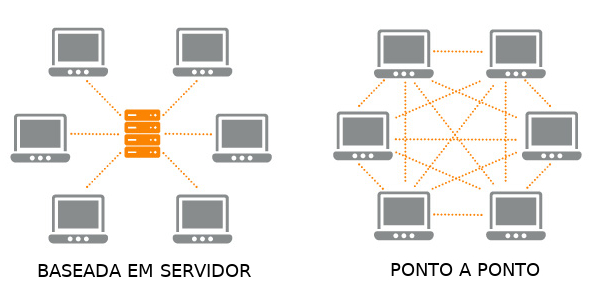
\includegraphics[width=\textwidth]{imagens/Server-based-vs-P2P-network.jpg}
	\caption{Rede com a arquitetura centralizada à esquerda e rede ponto a ponto à direita}
	Fonte: \cite{Wowza}
	\label{fig:redes}
\end{figure}

Na arquitetura centralizada, toda a rede fica dependente de um nó central, que fornecerá todos os recursos necessários para o funcionamento da rede. Esse nó detém todo o poder e controle, caso haja algum problema com ele, a rede ficará comprometida por completo. Já nas redes \textit{peer-to-peer}, isso não é um empecilho. Caso algum nó sofra com algum problema ou se desconecte voluntariamente da rede ou perca todas as informações, ninguém será afetado, todos continuarão realizando suas ações normalmente.

Apesar das vantagens, os sistemas ponto a ponto apresentam contrapartidas. Entre elas estão, principalmente, a integridade e confiança. Problemas estes que podem estar relacionados com falhas técnicas, nós mal intenciondos (usuários maliciosos), vulnerabilidade, integridade de informação, entre outros.
\section{Bitcoin}

O \textit{Bitcoin} geralmente é tratado como se fosse apenas uma moeda. Porém, o \textit{Bitcoin} é uma coleção de conceitos e tecnologias responsáveis por formar a base de todo um ecossistema um dinheiro digital. \cite{Antonopoulos2014} Dentro dessa variedade de conceitos que podem ser atribuídos a ele, podemos destacar três: (1) Um ativo digital (criptomoeda), (2) uma referência à tecnologia \textit{Blockchain} (livro-razão descentralizado) e (3) o protocolo que é executado sobre a tecnologia \textit{Blockchain} para descrever como os ativos são transferidos (\textit{softwares} que conduzem a transação) \cite{Swan2015}.

Todo esse sistema de pagamento de dinheiro digital foi lançado em 2009, sendo desenvolvido com um \textit{design} descentralizado e protegido por uma poderosa criptografia, tornando-o resiliente contra manipulações. \cite{Caetano2015} Os usuários possuem chaves que permitem com que eles provem a sua posse das moedas no decorrer das transações. Tais chaves são sempre armazenadas em uma carteira digital, a qual pode existir no computador do usuário, em sites de transações, em \textit{exchanges}, em \textit{hardwares}, ou em outras plataformas digitais. 

\section{Blockchain}

Assim, como o \textit{Bitcoin}, o \textit{Blockchain} também abrange um leque de significados, como: (1) uma terminologia para uma estrutura de dados, (2) o nome de um algoritmo, (3) um conjunto de tecnologias e (4) um termo abrangente para sistemas \textit{peer-to-peer} puramente distribuídos com uma área de aplicação comum.

Quando utilizado para nomear uma estrutura de dados, o termo refere-se a vários dados unidos em unidades chamadas de blocos. Tais blocos são conectados uns aos outros de forma encadeada, daí vem o nome \textit{Blockchain} (cadeia de blocos, em tradução livre). Quando atribuído a um algoritmo, o significado refere-se a um conjunto de instruções que lidam com o conteúdo de muitas estrutura de dados \textit{Blockchain} em um sistema \textit{p2p}. Ao se referir a um conjunto de tecnologias, o termo inclui a estrutura de dados, o algoritmo, tecnologias de criptografia e segurança os quais podem ser utilizados para prover integridade em sistemas puramente distribuídos ponto a ponto. E, diferente do significado anterior, a quarta atribuição ao termo é referente à um sistema distribuído como um todo, não unicamente a uma unidade de \textit{software} que faz parte desse tipo de sistema. \cite{Drescher2018}

O desenvolvimento desta tecnologia foi um avanço fundamental na ciência da computação, juntando cerca de quarenta anos de pesquisas em criptografia com vinte anos de pesquisas em moedas criptográficas. \cite{Swan2015} O Blockchain resolve um problema de longa data chamado “gasto duplo”. Este problema ocorre quando duas transações são aceitas com um montante que excede o valor antes disponível para gasto, ou seja, aquela quantia foi usada mais de uma vez.

Até o desenvolvimento do \textit{Blockchain}, o dinheiro digital não era escasso (assim como todos os outros recursos digitais), podendo ser copiados e replicados \textit{ad infinitum}, e não havia uma ­maneira de confirmar se aquele recurso já havia sido gasto sem que houvesse uma terceira parte envolvida para intermediar e realizar a sincronização entre todas as transações \cite{Swan2015}.

Para resolver o gasto duplo, o \textit{Blockchain} provê um mecanismo de confirmação e um livro-razão universal distribuído para que todos os nós (pontos) estejam informados e atualizados ao longo de cada transação. Cada informação nova adicionada na cadeia de blocos é armazenada em ordem cronológica, assim, fazendo com que o rastreamento seja feito de maneira simples. A cada 10 minutos um novo grupo de transações – ou seja, um bloco – é adicionado ao livro e todos os nós possuirão uma cópia do mesmo. Caso alguém tente usar o mesmo recurso mais de uma vez, será impossível, pois uma vez que a primeira operação dela foi iniciada, a mesma vai para um \textit{pool} de transações não confirmadas. Apenas a primeira das duas transações será confirmada e verificada pelos mineradores, enquanto a segunda será classificada como inválida e não terá confirmações suficientes para ser validada; e mesmo que as duas transações sejam feitas ao mesmo tempo, a que tiver mais confirmações dos mineradores (no mínimo seis, para que seis outros blocos sejam adicionados no topo do bloco que está sendo verificado) será a aceita.

A imagem abaixo mostra os passos para a realização de uma transação com \textit{Blockchain}. Primeiro, o usuário requisita uma transação. Em seguida, essa mesma requisição é transmitida para a rede, que será responsável por validar ou rejeitar o pedido de transação. Após isso, caso seja validada, ela é adicionada ao atual bloco de transações, o qual será encadeado com os outros blocos mais antigos, assim, confirmando a transação.

\begin{figure}[h]
	\centering
	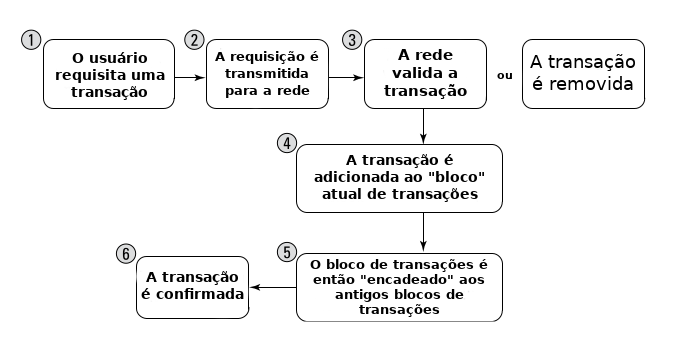
\includegraphics[width=\textwidth]{imagens/funcionamento-blockchain.png}
	\caption{Funcionamento do Blockchain}
	Fonte: \cite{Laurence2017}
	\label{fig:funcionamento-blockchain}
\end{figure}

A relação entre os sistemas \textit{p2p} e o \textit{Blockchain} é que o último serve para prover manter a integridade do primeiro sem que haja intermediação \cite{Drescher2018}.

\section{Exchanges}

As exchanges de criptoativos são plataformas digitais, com funcionamento
em tempo real que servem como intermediárias na compra, venda e troca dos mesmos, a fim de
facilitar o processo de aquisição. Elas costumam cobrar taxas nessas transações e organizar as 
informações de cada negociação em livros abertos. As exchanges são intermediários optativos, já
que, as criptomoedas podem funcionar de forma independente sem a necessidade de um intermediário envolvido no processo.

As seis \textit{exchanges} abordadas neste trabalho foram escolhidas com base no seu volume de transação e no nível de maturidade de sua \textit{API}. O volume é definido pela soma de todos os pares de mercado (\textit{market pairs}\footnote{\em Um \textit{market pair} é a cotação de duas moedas diferentes, com o valor de uma sendo cotado contra o valor de outra. O par é composto por uma moeda base e outra moeda de cotação.}) reportado pela corretora nas últimas vinte e quatro horas.

As informações a respeito do volume das corretoras são encontradas no \textit{Coin Market Cap}\footnote{\em https://coinmarketcap.com/rankings/exchanges/}, um \textit{site} que disponibiliza dados e gráficos em tempo real tanto das \textit{exchanges} quanto das criptomoedas existentes no mercado. No momento da escolha, as corretoras aqui analisadas estavam presentes entre as vinte primeiras posições no \textit{Coin Market Cap}.


\section{HTTP}

Projetado no início da década de 1990, o \textit{Hypertext Transfer Protocol} (Protocolo de Transferência de Hipertexto) é um protocolo de comunicação utilizado na transferência de documentos na \textit{Internet}. Ele garante a integridade dos dados transmitidos durante a comunicação. É por meio dele que as informações oriundas de servidores \textit{web} chegam de forma rápida, conveniente e confiável aos internautas, nos seus respectivos navegadores. O \textit{HTTP} segue o modelo de comunicação cliente-servidor, o qual o cliente inicia uma conexão com o servidor, realiza requisições e aguarda até receber alguma resposta.

\begin{figure}[h]
	\centering
	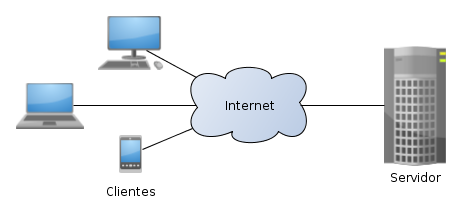
\includegraphics[width=\textwidth]{imagens/modelo-arquitetura-cliente-servidor.png}
	\caption{Modelo de arquitetura cliente-servidor}
	\cite{ClienteServidorWikipedia}
	\label{fig:modelo-arquitetura-cliente-servidor}
\end{figure}

\begin{figure}[h]
	\centering
	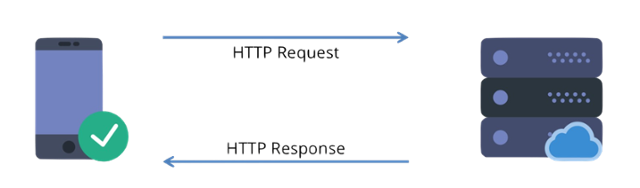
\includegraphics[width=\textwidth]{imagens/requisicao-http.png}
	\caption{Funcionamento de uma requisição HTTP}
	Fonte: \cite{HttpRequest}
	\label{fig:requisicao-http}
\end{figure}

Os servidores \textit{web} – também conhecidos como servidores \textit{HTTP} – são responsáveis por armazenar e prover todos os tipos de recursos \textit{web}: arquivos de texto, arquivos \textit{HTML}, arquivos de multimídia, etc.. O \textit{client} requisita ao \textit{server} o conteúdo desejado por meio de \textit{HTTP requests}  (requisições), e os servidores retornam os dados por meio de \textit{HTTP responses} (respostas) \cite{Gourley&Totty2002}, como mostrado na figura \ref{fig:requisicao-http}.

Além das características citadas, anteriormente, este protocolo é \textit{stateless}, ou seja, cada requisição é independente, mesmo que venham a ocorrer de forma simultânea e na mesma conexão cliente-servidor. Para o \textit{server}, cada \textit{request} é diferente, ele não guarda o estado das requisições anteriores, toda a informação é perdida.

\subsection{REST}

\textit{REST} é um acrônimo para \textit{Representational State Transfer} (Transferência de Estado Transacional), um estilo arquitetural para sistemas \textit{web} distribuídos a fim de facilitar a comunicação entre eles. Foi apresentado em 2000 por Roy Fielding, um dos autores da especificação do \textit{HTTP}, em sua tese de doutorado\footnote{\em https://www.ics.uci.edu/~fielding/pubs/dissertation/top.htm}. Nela, Roy sugeriu um conjunto de princípios, regras e \textit{constraints} que permitem o desenvolvimento de aplicações com interface bem definidas.
	
As aplicações desenvolvidas que seguem essa arquitetura são denominadas \textit{RESTful}, e seis princípios devem ser respeitados na implementação das mesmas:

\begin{itemize}
	\item \textbf{Cliente-servidor}: a portabilidade da interface do usuário e a escalabilidade do sistema  são melhoradas quando há uma separação do cliente, responsável pela interface, do servidor, que armazena as informações;
	\item \textbf{Stateless}: informações de sessão do usuário fica a cargo do cliente. Cada requisição para o servidor deve conter todas as informações necessárias para que ele entenda o \textit{request};
	\item \textbf{Armazenamento em cache}: requer que os dados em uma resposta sejam rotulados implícita ou explicitamente se podem ou não serem armazenados em \textit{cache}. Caso positivo, o cache do cliente poderá utilizar essas informações retornadas do servidor em outras requisições futuras;
	\item \textbf{Interface uniforme}: a fim de simplificar a arquitetura de todo o sistema, o \textit{REST} busca obter uma interface uniforme definindo quatro \textit{constraints}: identificação dos recursos, manipulação dos recursos através de representações, mensagens auto descritivas e hipermídia como motor do estado da aplicação;
	\item \textbf{Sistemas em camadas}: este modelo, também conhecido como \textit{layered systems}, permite que uma arquitetura seja composta de camadas hierárquicas, restringe o comportamento dos componentes de forma que cada um deles não possa acessar outras camadas além da qual eles estão interagindo no momento;
	\item \textbf{Código sob demanda}: este último princípio é optativo. Geralmente o usuário enviará as representações estáticas de recursos (\textit{JSON} ou \textit{XML}), porém, caso seja necessário, é possível retornar o código fonte executável para suportar parte da aplicação que está sendo desenvolvida.
\end{itemize}

\section{API}

\textit{Application Programming Interface} – Interface de Programação de Aplicações, em tradução livre – é um conjunto de definições, protocolos e ferramentas para o desenvolvimento e integração de \textit{softwares} de aplicações. Essa interface permite que o sistema possa se comunicar com produtos e serviços oferecidos por outras aplicações, dessa forma, simplificando e tornando mais flexível o processo de construção do sistema, consequentemente, gerando economia de tempo e de recursos.

Com as \textit{APIs}, a aplicação deixa disponível recursos, serviços e informações sem que haja uma perda na segurança e no controle, já que o acesso e as permissões serão especificadas pela equipe de desenvolvimento. Nos últimos anos, o \textit{REST} vem sendo o principal protocolo de padronização de \textit{APIs}.

\subsection{\textit{REST API: Design Rulebook}}

É o principal material utilizado neste trabalho como base para realizar as análises das \textit{APIs}. Segundo \cite{Masse:2016}, as regras servem para ajudar os desenvolvedores a construir \textit{RESTful APIs} consistentes que podem ser desfrutadas pelos usuários. Algumas delas tornaram-se padrões, de fato, outras era implícitas no protocolo \textit{HTTP}. Tais regras podem ser utilizadas por completo ou de forma separada, dependendo do contexto do serviço, e elas servem para responder algumas questões como:

\begin{itemize}
	\item Quando os caminhos da \textit{URI} devem ser nomeados com substantivos no plural?
	\item Quais métodos de requisição devem ser utilizados para atualizar o estado dos recursos?
	\item Como implementar operações diferentes do \textit{CRUD} nas \textit{URIs}?
	\item Qual é o código de \textit{status} \textit{HTTP} apropriado para um determinado cenário?
	\item Como gerenciar diferentes versões de uma representação do estado de um recurso?
	\item Como estruturar um \textit{hyperlink} em \textit{JSON}? 
\end{itemize}

\section{Trabalhos relacionados}

\subsection{\textit{API Management: An Architect’s Guide to Developing and Managing APIs for Your Organization}}

Este livro é um guia de como desenvolver, gerenciar e manter \textit{APIs} em sistemas corporativos. O autor aborda questões de segurança, ciclo de vida, documentação, padrões de projeto, controle de versão, monetização, \textit{analytics} e estratégias para testes de performance e testes de carga.

Na seção de seção de \textit{design} da interface da \textit{API}, princípios básicos do \textit{REST}, os verbos, os \textit{status codes}, a estrutura, convenções e boas práticas dos identificadores de recursos \textit{URIs}, versionamento, e outros detalhes importantes e necessários no projeto de construção de uma \textit{API}.

Segundo \cite{De2017}, as \textit{APIs} devem ser desenvolvidas para que tenham um longo ciclo de vida. Qualquer mudança acarreta em riscos de funcionamento para o cliente que a consome. Frequentes mudanças geralmente deixam usuários comuns e desenvolvedores frustrados. Utilizar padrões robustos na construção de \textit{APIs} ajuda a comunidade de desenvolvedores e pode salvar a companhia de ter despesas financeiras.

\subsection{\textit{REST API Development with Node.js: Manage and Understand the Full Capabilities of Successful REST Development}}

Assim como o trabalho anterior, neste livro o \cite{Doglio:2018} mostra todos os passos necessários para se desenvolver uma \textit{API} e lançá-la em um ambiente de produção. Nele, é feita uma introdução ao \textit{REST} e como desenvolver uma \textit{RESTful API} na linguagem \textit{Javascript} utilizando o \textit{framework Node.js}. A diferença encontra-se na abordagem das boas práticas de desenvolvimento de \textit{APIs}. O livro traz o conteúdo de forma mais superficial, não se aprofundando ou expondo os padrões minuciosamente. Por outro lado, o autor abordar o conteúdo didaticamente.

\subsection{\textit{API Design for C++}}

Este livro trata de forma mais profunda a construção de \textit{APIs} elegantes e robustas. Criar interfaces de alta qualidade é, portanto, uma habilidade essencial de engenharia e o foco central deste trabalho. \cite{Reddy2011}

Para auxiliar na performance, o autor utiliza a linguagem de programação \textit{C++}, que permite que a aplicação seja processada até mesmo em unidades de processamento gráfico (GPU). Alguns componentes para aumentar o desempenho das \textit{APIs} são considerados, entre eles: velocidade do tempo de compilação, velocidade do tempo de execução, sobrecarga da memória em tempo de execução, tamanho da aplicação e o tempo de inicialização.

Além do desempenho da aplicação, o livro aborda os diferentes tipos de \textit{patterns} de implementação e possui uma seção que trata da qualidade de uma \textit{API}, descrevendo as caracteríticas que uma boa aplicação deve ter, entre elas: modelagem do domínio do problema, esconder os detalhes de implementação, ser fácil de utilização, ser testada, documentada e estável.


% % \include{capitulos/coletando}

% % \include{capitulos/aplicando}

% % \include{capitulos/guiando}

% % \include{capitulos/experimentos}

% \chapter{Considerações Finais}
\label{chap:conclusao}
Corretoras de criptomoedas existem há menos de dez anos e, devido à necessidade de consultar informações e automatizar tarefas em tempo real, algumas delas já possuem uma \textit{API} para que seja possível acessar dados públicos e privados.

Desenvolvedores encontram dificuldade de lidar com tais \textit{APIs} por diferentes motivos, entre eles: documentação mal escrita e mal detalhada, erros inesperados, inconsistência de dados, ausência de tratamento de erros, limitações, entre outros.

Este trabalho apresenta uma análise comparativa das \textit{RESTful APIs} de seis diferentes \textit{exchanges} de criptomoedas baseado em padrões e boas práticas de desenvolvimento, objetivando servir como base para outros desenvolvedores que atuam desenvolvendo soluções para o mercado de criptoativos.

A fim de atingir os objetivos da pesquisa, o desenvolvimento foi dividido em três partes: escolha das regras que serão utilizadas como parâmetros, análise individual dos padrões e do funcionamento das \textit{APIs} conforme cada critério e levantamento das pontuações gerais obtidas pelas corretoras.

Na primeira fase, um escopo para definir as regras foi delimitado. Foram escolhidos os critérios mais básicos e necessários que todas as aplicações devem seguir, levando em consideração o contexto que essas \textit{APIs} estão inseridas. 

Na análise, o trabalho foi realizado de forma individual, para que houvesse um aprofundamento no estudo e nos testes de cada
\textit{exchange}. Além disso, foi realizada uma pesquisa a respeito das limitações de cada \textit{API REST},
servindo, no fim, como um complemento à análise.

E, por último, um resumo de cada conjunto de regras por categoria, detalhando o cumprimento das mesmas e aprofundando na comparação e nas causas que podem levar ou não ao cumprimento de tais regras.

Durante este estudo, foi possível notar que as equipes de desenvolvimento das corretoras pouco se preocupam com as boas práticas e os padrões definidos para aplicações \textit{RESTful}. Podendo isso ser prejudicial aos consumidores, que precisam desse serviço disponibilizado para desenvolver seus sistemas, e, até mesmo, à própria plataforma da \textit{exchange}, com dados irreais e outros possíveis erros.

No balanço total, a Binance foi a corretora que mais cumpriu as regras, seguida da Livecoin e da Huobi. Já a Bittrex, a Gate.io e a Poloniex, cumpriram menos da metade das regras, dessa forma, mostrando que as suas \textit{APIs} estão imaturas no quesito padronização do desenvolvimento.

\section{Limitações}

A principal limitação encontrada nesta pesquisa foi a falta de informações disponibilizadas pelas documentações das \textit{APIs}. Em algumas \textit{exchanges} analisadas, detalhes sobre os possíveis tipos de respostas de cada \textit{endpoint}, também sobre os \textit{status codes} e mensagens internas são omitidos. Em uma corretora específica, a Gate.io, sequer são informados os limites de requisições e o tempo de bloqueio após tal limite ser ultrapassado, dessa forma, dificultando os testes e as simulações realizadas.


\section{Trabalhos futuros}

O desenvolvimento de \textit{APIs} passa por diversos estágios, entre eles: gerenciamento, modelagem, documentação, versionamento, testes e governança. Por ser uma área vasta e complexa, a pesquisa pode, futuramente, ser estendida analisando a documentação escrita pelas corretoras e realizando testes unitários, de performance e de segurança

O estudo das \textit{exchanges} pode ser levado a outro patamar com o acréscimo de mais \textit{APIs} e com a inserção de mais um objeto de análise, os \textit{Websockets}, os quais, diferentemente das \textit{RESTful APIs}, estão menos presentes nas corretoras.

% % Bibliografia (arquivo Capitulos/Referencias.bib)

% \bibliography{capitulos/referencias}
% \bibliographystyle{abnt-alf}

% % Ap���ndice A (arquivo Includes/ApendiceA)
% % % Ap�ndice
\apendice
\chapter{Primeiro apêndice}

Os apêndices são textos ou documentos elaborados pelo autor, a fim de
complementar sua argumentação, sem prejuízo da unidade nuclear do trabalho.


% % Anexo A (arquivo Includes/AnexoA)
% % % Anexo
\anexo
\chapter{Primeiro anexo}

Os anexos são textos ou documentos não elaborado pelo autor, que servem de
fundamentação, comprovação e ilustração.


% % P���gina em branco
% \newpage

% \end{document}